%% ----------------------------------------------------------------
%% Thesis.tex -- MAIN FILE (the one that you compile with LaTeX)
%% ---------------------------------------------------------------- 

% Set up the document
\documentclass[a4paper, 11pt, oneside]{Thesis}  % Use the "Thesis" style, based on the ECS Thesis style by Steve Gunn
\usepackage[titletoc]{appendix}% https://ctan.org/pkg/appendix

\graphicspath{{Figures/}}  % Location of the graphics files (set up for graphics to be in PDF format)

% Include any extra LaTeX packages required
\usepackage[square, numbers, comma, sort&compress]{natbib}  % Use the "Natbib" style for the references in the Bibliography
%\usepackage{natbib}
\usepackage{verbatim}  % Needed for the "comment" environment to make LaTeX comments
\usepackage{vector}  % Allows "\bvec{}" and "\buvec{}" for "blackboard" style bold vectors in maths
\usepackage{placeins}

\usepackage{array}
\usepackage[table]{xcolor}
\usepackage{graphicx}
\usepackage{multirow}
\usepackage{pdflscape} % Added for landscape orientation of figures
\usepackage{rotating} % Added for rotated text in tables
\usepackage{multicol} % Added for multi-column layouts
\usepackage{enumitem} % Added for enhanced list environments
\hypersetup{urlcolor=blue, colorlinks=true}  % Colours hyperlinks in blue, but this can be distracting if there are many links.
\renewcommand{\bibname}{References}

%% ----------------------------------------------------------------
\begin{document}
\frontmatter	  % Begin Roman style (i, ii, iii, iv...) page numbering

% Set up the Title Page
\title  {ft\_transcendence}
 
\authors  {\texorpdfstring
            {\href{your web site or email address}{enrico@42abudhabi.ae}}
            { }
            }
\addresses  {\groupname\\\deptname\\\univname}  % Do not change this here, instead these must be set in the "Thesis.cls" file, please look through it instead
\date       {\today}
\subject    {}
\keywords   {}

\maketitle
%% ----------------------------------------------------------------

\setstretch{1.3}  % It is better to have smaller font and larger line spacing than the other way round

% Define custom page styles for chapter pages and regular pages
\fancypagestyle{chapterfirst}{%
  \fancyhf{} % Clear all headers and footers
  \fancyfoot[C]{\thepage} % Page number at bottom center
  \renewcommand{\headrulewidth}{0pt} % No header rule
}

\fancypagestyle{chapterrest}{%
  \fancyhf{} % Clear all headers and footers
  \fancyhead[L]{\leftmark} % Chapter number and title at top left
  \fancyhead[R]{\thepage} % Page number at top right
  \renewcommand{\headrulewidth}{0.4pt} % Header rule
}

% Format for chapter headers - important to define this before modifying the chapter command
\renewcommand{\chaptermark}[1]{\markboth{\chaptername\ \thechapter.\ #1}{}} 

% Modify chapter command to use chapterfirst style on first page
\makeatletter
\let\stdchapter\chapter
\renewcommand*{\chapter}{%
  \cleardoublepage % Start each chapter on a new page
  \thispagestyle{chapterfirst}% First page of chapter uses firstpage style
  \stdchapter
}
\makeatother

% Set the default pagestyle to chapterrest
\pagestyle{chapterrest}

%% ----------------------------------------------------------------
% Declaration Page required for the Thesis, your institution may give you a different text to place here
\clearpage  % Declaration ended, now start a new page
% The Abstract Page
\addtotoc{Abstract}  % Add the "Abstract" page entry to the Contents
\abstract{ 
\addtocontents{toc} {\vspace{1em}} % Add a gap in the Contents, for aesthetics

The growing challenge of creating secure, interactive web-based gaming applications has led to new approaches combining traditional web frameworks with blockchain technology and modern DevOps practices. Web-based gaming applications face significant challenges in delivering seamless multiplayer experiences while maintaining security, performance, and data integrity. The classic Pong game provides an ideal foundation to explore these challenges, raising the question of how modern web technologies can be leveraged to create a feature-rich, secure, and scalable gaming platform. ft\_transcendence is a modern, feature-rich clone of the classic Pong game implemented as a full-stack web application that addresses these challenges. Prior implementations of web-based Pong games have often lacked integration with modern security practices, blockchain technology, and containerized deployment strategies. Many existing solutions fail to address the security vulnerabilities inherent in web applications, particularly when running containerized services as root users. This project demonstrates the integration of real-time gameplay, secure authentication, on-chain tournament recording, and full DevOps automation within a Docker-Compose stack. The backend is powered by Django and PostgreSQL, exposing a clean RESTful API secured with JWT cookies and optional TOTP-based Two-Factor Authentication (2FA). Users can authenticate via 42 OAuth or traditional credentials with proper security measures including non-root container execution. The frontend, crafted using vanilla JavaScript and Bootstrap 5, delivers a responsive single-page application rendered on an HTML5 <canvas> element for immersive gameplay. Game modes include 1v1, AI opponents, 4-player multiplayer, and tournament brackets. Match and tournament data are stored both in PostgreSQL and on an Ethereum sidechain, ensuring immutability and verifiability. Static content and reverse proxying are handled by Nginx, which also enforces HTTPS using TLS. The system integrates centralized logging and monitoring through the ELK stack, and supports production-grade deployment via Docker and Makefiles. The implementation achieves cross-browser compatibility and accessibility for visually impaired users. This research demonstrates how combining traditional web technologies with blockchain solutions creates secure, verifiable gaming experiences while addressing critical security vulnerabilities through proper container user management. The architecture showcases a framework for building scalable web applications that maintain data integrity while enhancing user engagement through profile customization, friends lists, online status, and detailed match history.
}



\clearpage  % Abstract ended, start a new page
%% ----------------------------------------------------------------
\clearpage  % End of the Acknowledgements
%% ----------------------------------------------------------------

\pagestyle{chapterrest}  % Use our custom page style consistently throughout the document


%% ----------------------------------------------------------------
% Define frontmatter page style
\fancypagestyle{frontmatter}{%
  \fancyhf{} % Clear all headers and footers
  \fancyhead[L]{\emph{\leftmark}} % Set the left side page header
  \fancyhead[R]{\thepage} % Page number at top right
  \renewcommand{\headrulewidth}{0.4pt} % Header rule
}

% Table of Contents
\cleardoublepage % Start on a new page
\markboth{Contents}{} % Set the left mark for this section
\pagestyle{frontmatter} % Use the frontmatter style
\tableofcontents  % Write out the Table of Contents

%% ----------------------------------------------------------------
% List of Figures
\cleardoublepage % Start on a new page
\markboth{List of Figures}{} % Set the left mark for this section
\listoffigures  % Write out the List of Figures

%% ----------------------------------------------------------------
% List of Tables
\cleardoublepage % Start on a new page
\markboth{List of Tables}{} % Set the left mark for this section
\listoftables  % Write out the List of Tables

%% ----------------------------------------------------------------
% List of Abbreviations
\cleardoublepage % Start on a new page
\markboth{List of Abbreviations}{} % Set the left mark for this section
\chapter*{List of Abbreviations}  % Create a new unnumbered chapter for the abbreviations
\addcontentsline{toc}{chapter}{List of Abbreviations}  % Add this to the Table of Contents

% Use a more compact format with reduced spacing to fit on one page
\vspace{-5mm}
\begin{description}[leftmargin=3cm,labelwidth=2.5cm,itemsep=1pt,font=\normalfont]
\item[\textbf{2FA}] Two-Factor Authentication
\item[\textbf{CI/CD}] Continuous Integration and Continuous Delivery/Deployment
\item[\textbf{DOM}] Document Object Model
\item[\textbf{DevOps}] Development Operations
\item[\textbf{Git}] Global Information Tracker
\item[\textbf{JWT}] JSON Web Tokens
\item[\textbf{OAuth}] Open Authorization
\item[\textbf{OTP}] One-Time Password
\item[\textbf{SPA}] Single Page Application
\item[\textbf{SDLC}] Software Development Life Cycle
\item[\textbf{SSR}] Server-Side Rendering
\item[\textbf{SQL}] Structured Query Language
\item[\textbf{TLS}] Transport Layer Security
\item[\textbf{UI}] User Interface
\item[\textbf{URL}] Uniform Resource Locator
\item[\textbf{XSS}] Cross-Site Scripting
\end{description}

%% ----------------------------------------------------------------
% Reset the header for the main content
\cleardoublepage % Start main content on a new page
\pagestyle{chapterrest} % Use our custom page style
\renewcommand{\sectionmark}[1]{\markright{\thesection\ #1}} % Format for section headers



\setstretch{1.3}  % Return the line spacing back to 1.3



%% ----------------------------------------------------------------
\mainmatter	  % Begin normal, numeric (1,2,3...) page numbering
\pagestyle{chapterrest}  % Use our custom page style for chapter pages

% Include the chapters of the thesis, as separate files
% Just uncomment the lines as you write the chapters

%% Chapter 1
% This is an example chapter





\chapter{Introduction} % Write in your own chapter title
\section{Introduction}

This project, \textbf{ft\_transcendence}, delivers a modern, feature-rich clone of the classic Pong game implemented as a full-stack web application. The primary goal is to provide a highly interactive and accessible multiplayer gaming experience directly within a web browser, leveraging a Single-Page Application (SPA) architecture. By incorporating features such as user history tracking, matchmaking, and tournament brackets, the platform enhances user engagement through competitive play and detailed gameplay statistics.

The system ensures that user data, match history, and tournament results are securely stored and managed. Standard gameplay data is persisted in a \textbf{PostgreSQL} database, while tournament outcomes are additionally recorded immutably on an \textbf{Ethereum sidechain}, showcasing a novel approach to data integrity in online gaming. The application is built using modern web technologies and DevOps best practices, aiming for a responsive, scalable, and secure platform where users can engage in real-time contests.

Key technical components include a \textbf{Django backend} utilizing the Django Rest Framework (DRF) to expose a clean RESTful API, and a \textbf{Vanilla JavaScript frontend} employing ES6 modules and Bootstrap 5 for a responsive user interface rendered on an HTML5 `<canvas>` element. The entire application stack, including the backend, frontend, database, blockchain node, and monitoring tools, is orchestrated using \textbf{Docker and Docker-Compose}, facilitated by \textbf{Nginx} serving as a reverse proxy and handling HTTPS termination. Centralized logging and monitoring are integrated via the \textbf{ELK stack} (Elasticsearch, Kibana).

Standard user management features are robust, offering secure registration and login via \textbf{native credentials} or \textbf{42 Intra OAuth 2.0}. Authentication relies on \textbf{JWT cookies}, with optional \textbf{Time-based One-Time Password (TOTP) Two-Factor Authentication (2FA)} for enhanced security. User profiles allow for customization (including avatar uploads and unique display names), display online status, manage friends lists, and provide insights into gameplay statistics such as wins, losses, and match history. Access to detailed profiles and social features is restricted to logged-in users.

The platform offers diverse gameplay options, including \textbf{1-vs-1} matches against other online players, challenging an \textbf{AI opponent}, engaging in local \textbf{4-player multiplayer} matches, and participating in structured \textbf{tournaments} with persistent, on-chain results. Throughout development, emphasis was placed on performance, security, and inclusivity, including considerations for users with visual impairments and ensuring cross-browser compatibility.

This project aims to push the boundaries of web-based gaming applications by integrating real-time gameplay, secure authentication, blockchain technology, and comprehensive DevOps automation into a cohesive and engaging user experience.


\chapter{Project Goals and Requirements}
\label{ch:goals}

The primary objective of the ft\_transcendence project is to create a comprehensive and engaging web-based Pong game experience. This involves not only replicating the core gameplay but also integrating modern web technologies, robust security features, and advanced functionalities. The specific goals defined for this project are as follows:

\begin{itemize}
    \item \textbf{Deliver a Single-Page Application (SPA):} The game must be playable directly in the browser without requiring page reloads, offering a seamless user experience.
    
    \item \textbf{Provide Secure User Management:} Implement a secure system for user registration, login, and profile management. This includes:
    \begin{itemize}
        \item Native credential authentication (username/password).
        \item Integration with the 42 Intra OAuth 2.0 provider.
        \item Secure session management using JSON Web Tokens (JWT) stored in cookies.
        \item Optional Time-based One-Time Password (TOTP) Two-Factor Authentication (2FA) for enhanced security.
    \end{itemize}
    
    \item \textbf{Offer Multiple Game Modes:} Cater to different player preferences by providing several ways to play Pong:
    \begin{itemize}
        \item 1 vs 1 online matches against other registered users.
        \item 1 vs AI matches against a computer-controlled opponent.
        \item Local 4-player multiplayer on a single screen.
        \item Structured tournaments with bracket progression.
    \end{itemize}
    
    \item \textbf{Persist Data Securely and Reliably:} Store user data, match history, and tournament results using appropriate technologies:
    \begin{itemize}
        \item Utilize a \textbf{PostgreSQL} relational database for general application data, user profiles, and individual match results.
        \item Record final tournament results immutably on an \textbf{Ethereum sidechain} (using a Proof-of-Authority consensus mechanism) to ensure data integrity and verifiability.
    \end{itemize}
    
    \item \textbf{Expose a Clean RESTful API:} Develop a well-documented Application Programming Interface (API) using Django Rest Framework (DRF). This allows the frontend SPA to communicate with the backend and enables potential future development of alternative clients (e.g., command-line tools, mobile applications).
    
    \item \textbf{Implement Production-Grade DevOps Practices:} Ensure the application is easy to deploy, manage, and monitor using industry-standard tools and practices:
    \begin{itemize}
        \item Containerize all application components (frontend, backend, database, etc.) using \textbf{Docker}.
        \item Orchestrate the multi-container application stack using \textbf{Docker-Compose} for easy setup and deployment.
        \item Utilize \textbf{Nginx} as a reverse proxy to handle incoming traffic, serve static frontend assets, and manage HTTPS termination.
        \item Integrate centralized logging and monitoring using the \textbf{ELK stack} (Elasticsearch, Kibana) to provide insights into application performance and potential issues.
        \item Provide convenient management commands using a \textbf{Makefile}.
    \end{itemize}
\end{itemize}

These goals collectively aim to produce a polished, secure, and feature-rich web application that showcases proficiency in full-stack development, DevOps, and blockchain integration within the context of a familiar and engaging game.

\chapter{Software Development Life Cycle (SDLC)}
\label{ch:sdlc}

This chapter outlines our approach to developing the project following the Software Development Life Cycle (SDLC) methodology. We cover the key phases including requirement analysis, design, implementation, testing, and evolution (maintenance). Each phase builds upon the previous one, ensuring a systematic and comprehensive development process.

The Software Development Life Cycle (SDLC) for this project follows a modified Waterfall model, incorporating Agile elements to enhance flexibility and iterative improvements. While the Waterfall approach provided a structured framework for sequential stages like requirement analysis, design, implementation, and testing, we introduced Agile practices such as ongoing feedback and peer-reviewed GitHub pull requests (PRs). This process of PR reviews allowed team members to give feedback on each other's code, identify potential issues early, and ensure quality and consistency across different modules. By integrating peer-reviewed PRs, we facilitated continuous testing, collaborative refinement, and adherence to best practices throughout the development. This hybrid methodology helped us achieve a balance of systematic progression with opportunities for iteration and improvement based on team insights.

\section{Requirement Analysis}

Requirement Analysis is the first and one of the most crucial phases of the Software Development Life Cycle (SDLC). During this phase, the focus is on gathering detailed requirements and defining the project’s objectives. This phase helps ensure that the project starts on the right track, with a clear understanding of what needs to be built, why it is being built, and how it will be used. Proper requirement analysis sets the foundation for all subsequent stages of the software development process.
By understanding and addressing potential risks early, such as technical feasibility, resource constraints, or user expectations, the project can avoid delays or even a potential failure. Additionally,  proper documentation and agreement on requirements ensure that all members are on the same page, reducing miscommunication and conflicts later. 
Starting with a solid foundation minimizes misunderstandings and scope changes and sets the stage for successful project execution. In order to properly gather the requirements, it was necessary to choose which modules best fit the team skills and interests. Initially some modules were set, and others were flagged as “interested”, that the team would do according to the project development. 


\section{Modules Implemented}

After a careful analysis, the following core modules and features were implemented, aligning with the project goals:

\begin{enumerate}
    \item \textbf{Backend Framework:} Utilized Django (Python framework) to build a robust and scalable backend, providing RESTful APIs via Django Rest Framework (DRF).
    \item \textbf{Frontend Implementation:} Developed a Single-Page Application (SPA) using Vanilla JavaScript (ES6+) for interactivity and HTML5 Canvas for game rendering. Leveraged Bootstrap 5 as a toolkit for responsive design and UI components.
    \item \textbf{Database Integration:} Employed PostgreSQL as the primary relational database for storing user data, match history, and application settings, integrated via the Django ORM.
    \item \textbf{User Management and Authentication:} Implemented comprehensive user management features including secure registration, profiles (with avatars and stats), and friend lists. Supported multiple authentication methods: native credentials, 42 Intra OAuth 2.0.
    \item \textbf{Enhanced Security:} Integrated JWT (JSON Web Tokens) via \texttt{djangorestframework-simplejwt} for stateless session management (using secure HttpOnly cookies) and provided optional TOTP-based Two-Factor Authentication (2FA) using \texttt{django-otp}.
    \item \textbf{Core Gameplay (Pong):} Developed the classic Pong game with various modes:
        \begin{itemize}
            \item 1 vs 1 online matches.
            \item 1 vs AI opponent.
            \item Local multiplayer (up to 4 players).
            \item Structured tournaments with bracket display.
        \end{itemize}
    \item \textbf{Blockchain for Tournaments:} Integrated an Ethereum sidechain (Proof-of-Authority) to immutably record tournament results using Solidity smart contracts and Web3.py interaction from the backend.
    \item \textbf{Game Customization:} Provided options for users to customize certain aspects of their game experience (details may vary, e.g., potentially paddle appearance or simple settings).
    \item \textbf{DevOps and Containerization:} Utilized Docker and Docker Compose to containerize all services (backend, frontend, database, Nginx, ELK, Geth) for consistent deployment and orchestration.
    \item \textbf{Monitoring:} Integrated the ELK stack (Elasticsearch, Kibana) for centralized logging and application monitoring.
    \item \textbf{Accessibility Considerations:} Included features to enhance accessibility, such as support for keyboard navigation and considerations for visually impaired users (e.g., high-contrast options).
\end{enumerate}

\section{Design the System Architecture}
The Design Phase is the second major stage in the SDLC, where the focus transitions from defining system requirements to designing how the system will meet those requirements. The project architecture is divided into independent services, each running in Docker containers, to enhance scalability and maintainability.

For the database, \texttt{PostgreSQL} is selected to ensure data integrity and seamless integration with \texttt{Django}, while \texttt{Bootstrap} is utilized for creating a responsive and accessible UI design on the frontend.

In terms of security design, secure login methods, including 42 login or username, with Two-Factor Authentication (2FA) and JSON Web Tokens (JWT) for authentication, are implemented.

During this stage, the initial draft of the website workflow and the structure of page linkages were established in a group meeting. This draft outlined user navigation through the site, detailing the connections between different pages to ensure a coherent user experience. This early planning phase was crucial for aligning development efforts across various teams, such as frontend design, backend functionality, and game integration, setting the foundation for subsequent implementation stages.

\begin{figure}[H]
    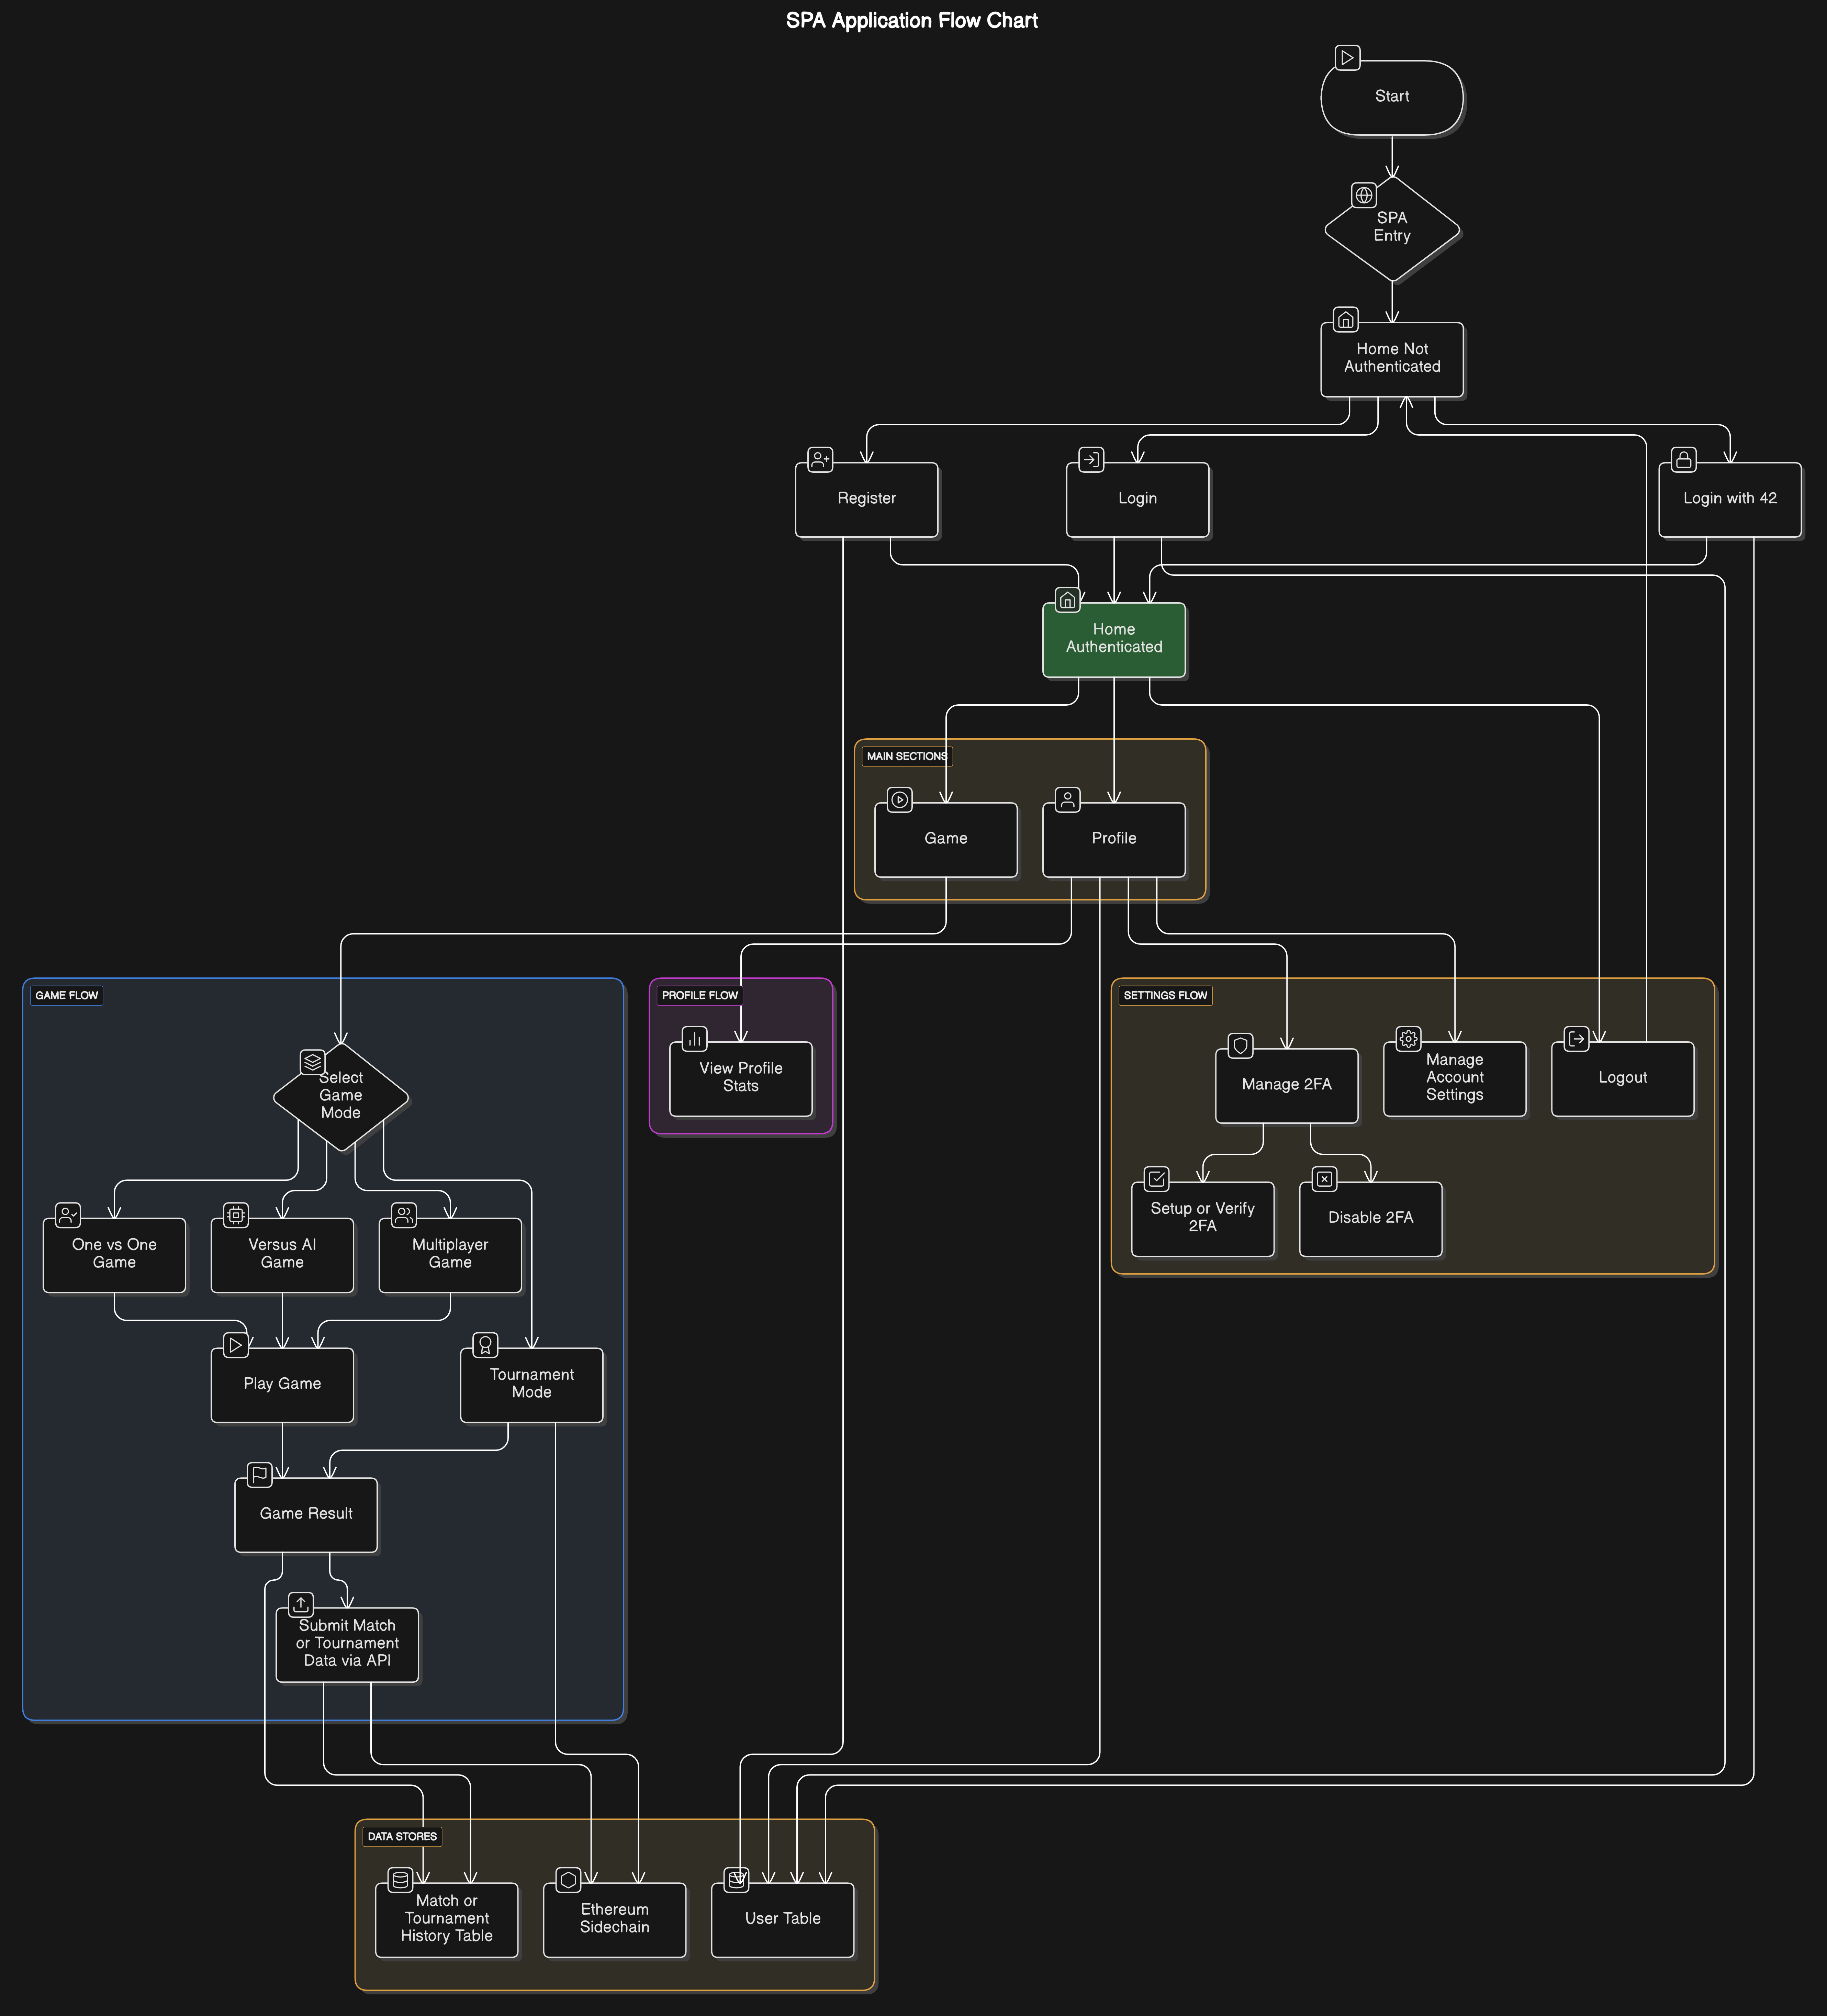
\includegraphics[width=1\linewidth]{Figures/images/workflow.png}
    \caption{Workflow}
    \label{fig:workflow}
\end{figure}


\section{Implementation}
The implementation step involves developing the actual code and functionality based on the design specifications. For this web application project, the implementation step was broken down into the following main aspects:
\begin{itemize}
    \item \textbf{Backend Development:} We developed the core functionality using Django, ensuring the backend supported all game features and incorporated robust security protocols. The backend manages user data securely, supports multiple game modes, and provides RESTful APIs for frontend interaction. The application is safeguarded against SQL injection and Cross-Site Scripting (XSS) attacks through Django's inherent security features. Specifically, Django mitigates SQL injection risks by automatically escaping user inputs and providing secure query methods. The framework's ORM functions such as \texttt{.filter()}, \texttt{.get()}, and \texttt{.exclude()} incorporate mechanisms that prevent execution of malicious SQL code. Additionally, we implemented non-root user execution in our Docker containers to address privilege escalation vulnerabilities.
    
    \item \textbf{Frontend Development:} We built a responsive user interface using Bootstrap 5, incorporating accessibility features such as high-contrast themes and keyboard navigation using the "tab" key. The frontend adapts seamlessly across different devices and screen sizes, offering an inclusive experience for users, including those with visual impairments. We implemented the SPA architecture using Vanilla JavaScript to minimize dependencies while maintaining performance.
    
    \item \textbf{Game Development:} We implemented the core Pong game mechanics with customization options for different skill levels and settings. This included developing interactive controls, configuring adjustable game parameters, and ensuring real-time responsiveness through optimized Canvas rendering. The game includes comprehensive user history tracking to record and display individual gameplay statistics.
    
    \item \textbf{User History and Matchmaking:} We integrated a user history tracking system to securely store game outcomes in PostgreSQL and ensure data is always up to date. These additions enhance user engagement by providing detailed gameplay statistics and facilitating seamless matchmaking for competitive play.
    
    \item \textbf{User Management and Authentication:} We implemented secure user management features with both native credentials and 42 OAuth authentication options, plus optional TOTP-based Two-Factor Authentication. Users can select unique display names, update their information, and upload avatars. Additional features include managing friend lists, viewing online status, and accessing user profiles with comprehensive statistics. All user management functionalities comply with best practices for secure authentication using JWT stored in HttpOnly cookies.
    
    \item \textbf{Development Workflow:} To enable simultaneous work across different components, we implemented a branching strategy on GitHub where each task had its dedicated branch. This approach allowed team members to work independently while preserving the integrity of the main branch. Before merging changes, a peer review process ensured code quality and caught potential issues early. Figure \ref{fig:workflow} illustrates this workflow from our development period (February to April 2025), demonstrating how multiple branches facilitated collaborative development and quality assurance.
\end{itemize}

\section{Testing the application and its functionalities}

Testing phase in the SDLC ensures that the web application is functional, secure, user-friendly, and meets all requirements. Focusing on Pong game web application, testing can be broken down into several types, each targeting different aspects of the system:
\begin{itemize}
    \item \textbf{Unit Testing:} Test individual components of the application in isolation to ensure their functionality is correct. Examples include verifying user authentication mechanisms, game logic (such as ball physics and paddle movements in Pong), and database interactions. These tests validate core functionality like game rules, user input handling, and match outcome determination.
    
    \item \textbf{Integration Testing:} After unit testing, it is necessary to test the interactions between multiple components. Integration testing includes verifying the communication between the frontend and backend (e.g., submitting a login request and receiving the correct response, game management, authentication, user profiles), and ensuring data is correctly stored, retrieved, updated, and deleted from the PostgreSQL database. It was also necessary to perform tests to confirm that the user history and matchmaking system of the game were operating seamlessly, and data flows correctly across services.
    
    \item \textbf{Functional Testing:} The main goal is to verify that the application meets all functional requirements and works as intended. This is done by testing the game functionality (e.g., in the Pong game, issues like ball collision detection, paddle movement, multiplayer synchronization, adjusting ball and paddle speed, difficulty levels, and sound settings should be analyzed). For authentication and security, it is necessary to check if both login methods (42 login and username), 2FA setup, and JWT session management are properly working, as well as if a non-logged user can access the content restricted to a logged user. In addition, the logout option was also tested to ensure that the session was properly finished. Lastly, user management features like user registration, profile updates, password resets, and tournament participation were analyzed.
    
    \item \textbf{Usability Testing:} This next step evaluates the application's user interface and experience, ensuring it is intuitive and accessible for users. The main tests were focused on testing the web application on different devices (desktop, tablet, mobile) to ensure the UI is responsive and easy to use, and checking that all accessibility features (e.g., high-contrast colors, keyboard navigation) work correctly and comply with accessibility standards. After that, the focus shifted to gathering feedback from users on the game's interface, navigation, and overall experience to identify potential improvements.
    
    \item \textbf{Compatibility Testing:} The goal is to ensure the application functions consistently across different environments. For this application, the browsers “Chrome” (last available version) and “Firefox” were chosen, and in this sense, all tests were performed on both browsers.
\end{itemize}

In addition to the tests mentioned above, CI/CD was integrated as an automation tool within the GitHub (Figure 2) workflow to prevent commits that would fail the build. This approach proved highly effective, minimizing rework and ensuring that each merge met the minimum standards required for committing to the main branch.


% \section{Testing the application}
% We periodically tested the code after each stage of code implementation to ensure that the code was running properly before moving on to the next stage. This involved a variety of tests, including unit testing to validate individual components, integration tests to assess how different parts of the system worked together, and user tests to gather feedback from real users. This testing strategy allowed us to identify and resolve bugs early, ensuring a smoother development process as we built the code.

% \section{Future improvements}
% After deployment, we need to focus on system maintenance and consider how we can update the game. This includes monitoring performance, addressing any issues that arise, and implementing enhancements based on user feedback. We should also plan for regular updates to introduce new features, fix bugs, and ensure the game remains engaging and enjoyable for players.


\chapter{Elements of SDLC}

\section{SDLC Methodology}

The Software Development Life Cycle (SDLC) for this project followed a hybrid approach, combining the structured framework of the Waterfall model with Agile elements for flexibility. While Waterfall provided sequential stages (requirement analysis, design, implementation, testing), Agile practices like ongoing feedback and peer-reviewed GitHub pull requests (PRs) were integrated. This PR review process allowed team members to assess code, identify issues early, and ensure quality and consistency. This hybrid methodology balanced systematic progression with iterative refinement based on team collaboration and insights.

\section{Gantt Chart}

% Force proper figure numbering once before the figure
\renewcommand{\thefigure}{3.\arabic{figure}}

% Full page figure with rotated image on a separate page
\begin{figure}[p]
    \centering
    % Rotate the image 90 degrees 
    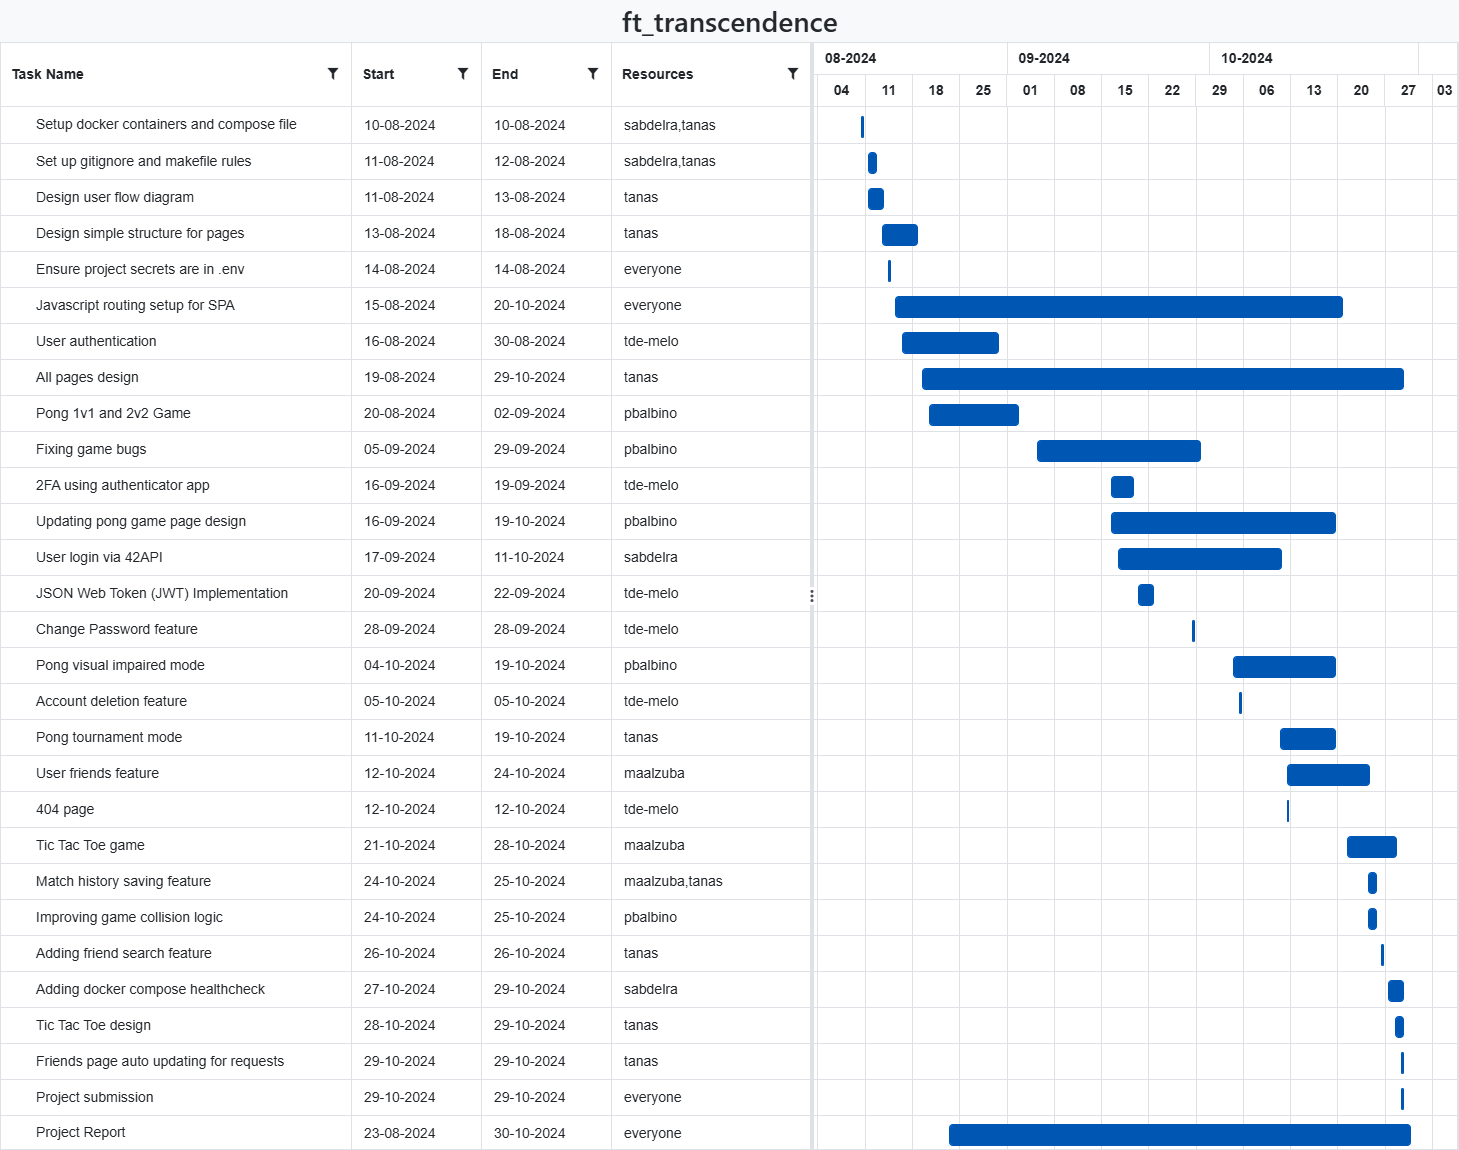
\includegraphics[angle=90, width=1\textwidth, height=1\textheight, keepaspectratio]{Figures/images/gantt-chart.png}
    \caption{Gantt Chart}
    \label{fig:gantt-chart}
\end{figure}


\clearpage
% Begin explanatory text on a new page
The Gantt Chart (Figure \ref{fig:gantt-chart}) delineates the project timeline, outlining tasks, dependencies, and milestones, thereby mapping the project's progression through each phase of the Software Development Life Cycle (SDLC).

This Gantt chart outlines the project timeline for \textbf{ft\_transcendence}, showing tasks, their durations, and assigned resources. It spans from August to October 2024, covering development milestones like setting up the \textbf{Docker environment} with \textbf{Docker-Compose}, designing user interfaces using \textbf{Bootstrap 5}, and implementing essential features such as user authentication (\textbf{Native Credentials, 42 OAuth, JWT, TOTP 2FA}). The project includes building the main Pong game modes (\textbf{1v1, vs AI, 4-player local, Tournaments}), integrating \textbf{Blockchain} for tournament storage, setting up the \textbf{ELK stack} for monitoring, and implementing user features like friend management, match history, and account settings. Key phases involve testing, debugging, and updating, with the planned submission date due by October 29, 2024. Various team members are responsible for specific tasks, ensuring collaborative progress throughout the timeline.

\section{Risk Register and Risk Matrix}

\subsection{Risk Register}
To ensure project success, we identified and managed potential risks through a systematic risk assessment process. The Risk Register documents all identified risks, their impact, probability, and mitigation strategies.

\begin{table}[H]
\centering
\begin{tabular}{|p{0.5cm}|p{3cm}|p{2.5cm}|p{2.5cm}|p{3cm}|p{2cm}|}
\hline
\rowcolor{gray!30}
\textbf{ID} & \textbf{Risk Description} & \textbf{Probability} & \textbf{Impact} & \textbf{Mitigation Strategy} & \textbf{Owner} \\ \hline

R1 & Technical complexity of integrating blockchain & Medium & High & Early research and prototyping; dedicated team member & Development Team \\ \hline

R2 & Real-time gameplay latency issues & High & High & Implement efficient algorithms, stress testing, optimize network code & Game Dev Team \\ \hline

R3 & Security vulnerabilities in authentication & Medium & Critical & Code reviews, security best practices, JWT token handling & Security Team \\ \hline

R4 & Docker orchestration complexity & Medium & Medium & Early setup, documentation, pair programming & DevOps Team \\ \hline

R5 & Scope creep due to additional game features & High & Medium & Clear requirements, regular reviews, prioritization & Project Manager \\ \hline

R6 & Integration issues between frontend and backend & Medium & High & API specification first, mock endpoints, continuous integration & Integration Team \\ \hline

R7 & Team member unavailability & Low & Medium & Cross-training, documentation, distributed knowledge & Team Lead \\ \hline

R8 & Browser compatibility issues & Medium & Medium & Cross-browser testing, progressive enhancement & UI/UX Team \\ \hline

R9 & Performance issues with ELK stack & Low & Low & Monitoring, resource allocation, performance tuning & DevOps Team \\ \hline

R10 & Incomplete or changing requirements & Medium & High & Regular stakeholder reviews, agile approach & Project Manager \\ \hline
\end{tabular}
\caption{Risk Register for the ft\_transcendence Project}
\label{table:risk-register}
\end{table}

\subsection{Risk Matrix}

The Risk Matrix provides a visual representation of the risks based on their probability and impact, helping prioritize risk mitigation efforts.

\begin{figure}[H]
\centering
\begin{tabular}{|p{2.5cm}|p{2.5cm}|p{2.5cm}|p{2.5cm}|p{2.5cm}|p{2.5cm}|}
\hline
\multicolumn{6}{|c|}{\textbf{RISK MATRIX}} \\
\hline
\multirow{6}{*}{\rotatebox[origin=c]{90}{\textbf{Probability}}} & 
\textbf{Very High} & Low Risk & Moderate Risk & \cellcolor{yellow!40}High Risk (R5) & \cellcolor{red!40}Critical Risk \\ \cline{2-6}
& \textbf{High} & Low Risk & \cellcolor{yellow!40}Moderate Risk & \cellcolor{red!40}High Risk (R2) & \cellcolor{red!40}Critical Risk \\ \cline{2-6}
& \textbf{Medium} & \cellcolor{green!30}Low Risk (R9) & \cellcolor{yellow!40}Moderate Risk (R4) & \cellcolor{yellow!40}High Risk (R1, R6, R10) & \cellcolor{red!40}Critical Risk (R3) \\ \cline{2-6}
& \textbf{Low} & \cellcolor{green!30}Low Risk & \cellcolor{green!30}Low Risk (R7) & \cellcolor{yellow!40}Moderate Risk (R8) & \cellcolor{yellow!40}High Risk \\ \cline{2-6}
& \textbf{Very Low} & \cellcolor{green!30}Low Risk & \cellcolor{green!30}Low Risk & \cellcolor{green!30}Low Risk & \cellcolor{yellow!40}Moderate Risk \\ \hline
& & \textbf{Low} & \textbf{Medium} & \textbf{High} & \textbf{Critical} \\ \cline{2-6}
& & \multicolumn{4}{c|}{\textbf{Impact}} \\ \hline
\end{tabular}
\caption{Risk Matrix showing probability vs. impact}
\label{fig:risk-matrix}
\end{figure}



\section{Functional Requirements}
\subsection*{User Authentication and Management}
\begin{itemize}
    \item Secure registration, login, and profile management.
    \item Support for multiple authentication mechanisms: Native username/password, 42 Intra OAuth 2.0, and optional TOTP-based Two-Factor Authentication (2FA).
    \item User profile management features, including unique display names, avatar uploads, and online status visibility.
    \item Friends list management (add, remove, view status).
\end{itemize}

\subsection*{Gameplay and Game Modes}
\begin{itemize}
    \item Core Pong gameplay implemented on HTML5 Canvas.
    \item Multiple game modes:
        \begin{itemize}
            \item 1 vs 1: Online match against another registered user.
            \item 1 vs AI: Match against a computer-controlled opponent.
            \item Local Multiplayer: Up to 4 players on the same screen.
            \item Tournament: Knockout bracket competition among registered users.
        \end{itemize}
\end{itemize}

\subsection*{Match History and Statistics}
\begin{itemize}
    \item Tracking and storing user gameplay statistics, including wins, losses.
    \item Displaying match history for logged-in users.
    \item Recording tournament results in PostgreSQL and immutably on the Ethereum sidechain.
\end{itemize}

\subsection*{Accessibility Features}
\begin{itemize}
    \item Considerations for visually impaired users (e.g., high-contrast options, clear UI elements).
    \item Keyboard navigation support for gameplay and interface interaction.
\end{itemize}

\section{Technical Requirements}
\section*{Software Specifications}

\subsection*{Operating System}
\begin{itemize}
    \item \textbf{Server Deployment}: Linux-based distribution (e.g., Debian, Ubuntu) is recommended for hosting Docker containers.
    \item \textbf{Development/Client}: Cross-platform compatibility (Linux, macOS, Windows) for development and playing via supported web browsers.
\end{itemize}

\subsection*{Programming Languages, Frameworks, and Libraries}
\begin{itemize}
    \item \textbf{Backend}: Python 3 with Django 5 framework. Django Rest Framework (DRF) for API development. Libraries include `djangorestframework-simplejwt` for JWT authentication and `django-otp` for 2FA.
    \item \textbf{Frontend}: Vanilla JavaScript (ES6+), HTML5, CSS3. Bootstrap 5 for responsive UI components and layout.
    \item \textbf{Blockchain Interaction}: Web3.py library for interacting with the Ethereum sidechain from the backend (or helper scripts).
\end{itemize}

\subsection*{Database and Data Storage}
\begin{itemize}
    \item \textbf{Primary Database}: PostgreSQL (Version 15 specified) for storing user data, match history, game settings, etc.
    \item \textbf{Blockchain}: Local Ethereum Proof-of-Authority (POA) sidechain (using Geth) for immutable storage of tournament results. Smart contracts developed in Solidity (details likely in `Blockchain/` directory).
\end{itemize}

\subsection*{Web Server and Reverse Proxy}
\begin{itemize}
    \item Nginx: Used as a reverse proxy to route traffic to the Django backend (via Gunicorn or similar WSGI server), serve static frontend files (JS, CSS, images), and handle TLS/SSL termination for HTTPS.
\end{itemize}

\subsection*{Containerization and Orchestration}
\begin{itemize}
    \item Docker: To containerize each service (frontend, backend, database, Nginx, ELK, blockchain node).
    \item Docker-Compose: To define and manage the multi-container application stack.
\end{itemize}

\subsection*{Authentication and Security Mechanisms}
\begin{itemize}
    \item JSON Web Tokens (JWT): Used for stateless session management via secure HTTP-only cookies.
    \item Two-Factor Authentication (2FA): TOTP-based 2FA support via `django-otp`.
    \item OAuth 2.0: Integration with 42 Intra's OAuth service.
    \item TLS/SSL: Encryption for all communication via HTTPS, handled by Nginx.
\end{itemize}

\subsection*{Monitoring and Logging}
\begin{itemize}
    \item ELK Stack: Elasticsearch (Version 7 specified) for log aggregation and indexing, Kibana (Version 8 specified) for visualization and analysis. Log shipping likely handled by Filebeat or integrated Django logging.
\end{itemize}

\section*{Hardware Specifications}
\subsection*{Server Requirements (Development/Small Scale)}
\begin{itemize}
    \item Processor: Modern multi-core CPU.
    \item Memory: Minimum 8 GB RAM (16 GB+ recommended, especially with ELK stack).
    \item Storage: SSD recommended (minimum 50-100 GB, depending on data volume and logs).
    \item Network: Standard internet connectivity.
\end{itemize}
*Note: Production requirements would depend heavily on user load.*

\subsection*{Client Requirements}
\begin{itemize}
    \item Device: Desktop, laptop with modern web browser.
    \item Browser: Latest versions of Chrome or Firefox recommended.
    \item Network: Stable internet connection for real-time gameplay.
\end{itemize}

\section*{System Architecture}
\subsection*{Client Layer (Frontend SPA)}
The frontend is a Single-Page Application (SPA) responsible for rendering the user interface, handling user interactions, and managing client-side game logic. Technologies:
\begin{itemize}
    \item Framework/Libraries: Vanilla JavaScript (ES6+), Bootstrap 5.
    \item Structure: HTML templates, CSS3 for styling.
    \item Rendering: Client-side rendering. Game logic executed directly in the browser, primarily using the HTML5 Canvas API for Pong gameplay.
    \item API Communication: Uses Fetch API or similar to interact with the backend REST API for data retrieval, user actions, and submitting game results.
    \item Authentication Handling: Manages JWT tokens received from the backend (stored securely, likely in HttpOnly cookies handled by the browser).
\end{itemize}

\subsection*{Application Layer (Backend API)}
The backend provides the RESTful API, manages business logic, handles user authentication, interacts with the database and blockchain, and integrates with monitoring systems. Technologies:
\begin{itemize}
    \item Framework: Django 5 (Python 3).
    \item API: Django Rest Framework (DRF) for creating API endpoints.
    \item Authentication: Handles user registration, login (native, OAuth), JWT generation/validation (`djangorestframework-simplejwt`), and 2FA logic (`django-otp`).
    \item Database Interaction: Uses Django ORM to communicate with the PostgreSQL database.
    \item Blockchain Interaction: May trigger helper scripts (`Web3.py`) to interact with the Ethereum sidechain for storing tournament data.
    \item Logging: Integrates with the ELK stack for centralized logging.
    \item WSGI Server: Typically runs behind Nginx using a WSGI server like Gunicorn (though not explicitly mentioned in README, it's standard for Django deployment).
\end{itemize}

\subsection*{Data Layer (Persistence)}
The data layer ensures persistent storage of application data using both relational and blockchain technologies. Technologies:
\begin{itemize}
    \item Relational Database: PostgreSQL 15 for user accounts, profiles, settings, individual match history, etc.
    \item Blockchain Database: Ethereum sidechain (Geth node running POA) for immutable recording of official tournament outcomes via smart contracts.
\end{itemize}

\subsection*{Infrastructure Layer (Orchestration and Hosting)}
This layer encompasses the tools and services used for deployment, management, and operation of the application stack. Technologies:
\begin{itemize}
    \item Containerization: Docker packages each component (frontend, backend, Postgres, Nginx, ELK, Geth) into isolated containers.
    \item Orchestration: Docker-Compose defines the relationships and configurations for running the multi-container application.
    \item Reverse Proxy / Web Server: Nginx manages incoming HTTPS traffic, routes requests to the appropriate backend service, serves static frontend assets, and handles SSL/TLS termination.
    \item Monitoring: ELK Stack (Elasticsearch, Kibana) provides infrastructure for log aggregation and analysis.
\end{itemize}

\subsection*{Communication and Networking}
\begin{itemize}
    \item Internal Communication: Services within the Docker network communicate over a private network defined by Docker-Compose.
    \item External Communication: All external client communication occurs over HTTPS (port 443), managed by Nginx.
    \item API Calls: Frontend communicates with the backend via RESTful HTTP requests to the API endpoints.
    \item Blockchain Calls: Backend (or scripts triggered by it) communicates with the Geth node via RPC calls (typically over HTTP or IPC).
\end{itemize}

\section{Non-functional Requirements}
Non-functional requirements define the quality attributes and constraints of the system.

\subsection*{Performance}
\begin{itemize}
    \item \textbf{Responsiveness}: The SPA frontend should provide a smooth user experience with minimal delays during navigation and interaction. Game rendering on the Canvas should be efficient to maintain playable frame rates.
    \item \textbf{Latency}: Network latency for real-time 1v1 games should be minimized, although the current implementation seems focused on client-side rendering with results submitted post-game. API response times should be reasonably fast.
    \item \textbf{Load Handling}: The system (especially Nginx and the Django backend) should be capable of handling a moderate number of concurrent users, scalable via Docker if needed.
\end{itemize}

\subsection*{Security}
\begin{itemize}
    \item \textbf{Authentication}: Secure mechanisms for login (native, 42 OAuth) and session management (JWT over HTTPS, HttpOnly cookies).
    \item \textbf{Authorization}: Proper checks to ensure users can only access their own data and perform actions they are permitted to.
    \item \textbf{Data Protection}: Use of HTTPS (TLS/SSL) for all external communication. Sensitive data in the database should be handled securely (e.g., password hashing via Django). Input validation to prevent common web vulnerabilities (XSS, SQL Injection) provided by Django/DRF.
    \item \textbf{Infrastructure Security}: Containers should run with non-root users. Network policies within Docker can restrict communication between containers.
    \item \textbf{2FA}: Optional TOTP-based 2FA provides an additional security layer.
\end{itemize}

\subsection*{Reliability}
\begin{itemize}
    \item \textbf{Availability}: The application should be available with minimal downtime. Docker and Nginx help manage service availability.
    \item \textbf{Data Integrity}: PostgreSQL ensures relational data integrity. Blockchain provides immutability for tournament records.
    \item \textbf{Fault Tolerance}: Containerized architecture allows individual services to be restarted if they fail. Error handling should be robust in both frontend and backend.
    \item \textbf{Backup and Recovery}: Regular backups of the PostgreSQL database are crucial (mentioned as a mitigation strategy).
\end{itemize}

\subsection*{Scalability}
\begin{itemize}
    \item \textbf{Component Scaling}: Docker-Compose allows scaling individual services (e.g., adding more backend instances) if necessary, although load balancing setup might need adjustment.
    \item \textbf{Database Scaling}: PostgreSQL offers various scaling options if needed in the future.
    \item \textbf{Stateless Backend}: Using JWT promotes a stateless backend architecture, which generally scales better horizontally.
\end{itemize}

\subsection*{Maintainability}
\begin{itemize}
    \item \textbf{Modularity}: The project is divided into distinct components (Frontend, Backend, Blockchain, Infrastructure) and containerized services, promoting separation of concerns.
    \item \textbf{Code Quality}: Adherence to coding standards and use of frameworks (Django, Bootstrap) aids maintainability.
    \item \textbf{Configuration Management}: Environment variables (`.env` file) are used for configuration, separating code from configuration.
    \item \textbf{DevOps Automation}: Makefile and Docker-Compose simplify build, deployment, and management tasks.
\end{itemize}

\subsection*{Usability and Accessibility}
\begin{itemize}
    \item \textbf{User Interface}: The UI, built with Bootstrap, should be intuitive and easy to navigate.
    \item \textbf{Responsiveness}: The application should adapt to different screen sizes (desktops primarily, given the game type).
    \item \textbf{Accessibility}: Conscious effort to include features for visually impaired users (high contrast, keyboard navigation) as stated in goals.
\end{itemize}

\section{Implementation}
The implementation phase involved developing the actual code and functionality based on the design specifications. Key aspects included:
\begin{itemize}
    \item \textbf{Backend Development:} Core functionality was built using Django and Django Rest Framework (DRF), providing a secure RESTful API. This included managing user data (PostgreSQL), handling authentication (Native, 42 OAuth, JWT, 2FA), supporting multiple Pong game modes, and ensuring security against common vulnerabilities like SQL injection and XSS through Django's built-in features.
    \item \textbf{Frontend Development:} A responsive Single-Page Application (SPA) interface was built using Vanilla JavaScript, HTML5, and CSS3, leveraging Bootstrap 5 for layout and components. Accessibility features like high-contrast themes and keyboard navigation were incorporated. The frontend interacts with the backend API and uses the HTML5 Canvas for rendering the Pong game dynamically.
    \item \textbf{Game Development:} Pong game mechanics were implemented using JavaScript and Canvas, including ball/paddle physics, scoring, and real-time updates (potentially via WebSockets, although not explicitly detailed in prior context). Game modes (1v1, vs AI, 4-player local, Tournament) were developed.
    \item \textbf{Blockchain Integration:} Smart contracts (Solidity) were developed and deployed to a local Ethereum sidechain (Geth) to immutably record tournament results. Backend interaction was handled using Web3.py.
    \item \textbf{User History and Statistics:} A system was integrated to track and display user match history and statistics (wins/losses), stored primarily in PostgreSQL.
    \item \textbf{User Management and Authentication:} Secure user registration, login (Native, 42 OAuth), profile management (display name, avatar), friends list, and TOTP 2FA were implemented. JWTs, managed via secure HttpOnly cookies, were used for session management.
    \item \textbf{DevOps and Deployment:} The entire application (Backend, Frontend, PostgreSQL, Nginx, ELK, Geth node) was containerized using Docker and orchestrated with Docker Compose. Nginx served as a reverse proxy and static file server. The ELK stack was configured for centralized logging and monitoring.
    \item \textbf{Collaborative Workflow:} GitHub branches were used for parallel development (e.g., backend, frontend, game features). Peer reviews were conducted on Pull Requests before merging to the main branch to maintain code quality.
\end{itemize}

\section{Testing}
The testing phase ensured the application's functionality, security, usability, and adherence to requirements. Key testing types included:
\begin{itemize}
    \item \textbf{Unit Testing:} Verifying individual components like authentication logic, specific API endpoints, Canvas rendering functions, and game rule implementations (e.g., ball collision, scoring) in isolation.
    \item \textbf{Integration Testing:} Testing interactions between components, such as frontend API calls to the backend for login/registration, fetching user profiles, submitting game results, database interactions (PostgreSQL CRUD operations), and backend communication with the Ethereum sidechain.
    \item \textbf{Functional Testing:} Validating end-to-end features against requirements. This involved testing all Pong game modes, user registration/login flows (Native, OAuth, 2FA), profile updates, friend management, tournament creation/participation, and ensuring restricted content access controls worked correctly.
    \item \textbf{Usability Testing:} Evaluating the user interface and experience for intuitiveness and accessibility. Testing responsiveness across different screen sizes (desktop, tablet, mobile) using Bootstrap, checking keyboard navigation, and verifying accessibility features for visually impaired users.
    \item \textbf{Compatibility Testing:} Ensuring consistent functionality across target browsers (latest Chrome and Firefox).
    \item \textbf{Security Testing:} Reviewing implementations for common web vulnerabilities (though specific penetration testing might not have been performed), verifying JWT handling, 2FA enforcement, and general adherence to security best practices mentioned in mitigation strategies.
    \item \textbf{CI/CD Integration:} Using GitHub Actions to automate checks (e.g., linters, basic tests) to prevent merging failing code into the main branch.
\end{itemize}

\section{Evolution}
This phase focuses on maintaining and enhancing the software post-initial deployment.
\subsection*{Backend Development}
\begin{itemize}
    \item \textbf{Initial Phase:} Focused on core Django/DRF setup, basic user auth, and foundational API endpoints for Pong.
    \item \textbf{Intermediate Phase:} Expanded to support multiple game modes, integrated 42 OAuth and 2FA, developed blockchain interaction logic (Web3.py), and refined APIs based on frontend needs.
    \item \textbf{Current Phase:} Provides a comprehensive API managing users, game logic, statistics, tournaments (with blockchain logging), and authentication, running within a Dockerized environment integrated with ELK.
\end{itemize}

\subsection*{Frontend Development}
\begin{itemize}
    \item \textbf{Initial Phase:} Basic SPA structure with Vanilla JS, Bootstrap layout, initial Canvas implementation for Pong.
    \item \textbf{Intermediate Phase:} Refined UI/UX based on feedback, improved responsiveness, enhanced Canvas rendering, integrated API calls for dynamic data, added accessibility features.
    \item \textbf{Current Phase:} Delivers an interactive SPA experience with real-time updates, customizable settings, smooth navigation, robust game interface via Canvas, and accessibility considerations.
\end{itemize}

\subsection*{Game Development}
\begin{itemize}
    \item \textbf{Initial Phase:} Developed core Pong mechanics on Canvas (ball/paddle movement, collision, scoring).
    \item \textbf{Intermediate Phase:} Added different game modes (1v1, AI, 4-player, Tournament), improved real-time responsiveness, added basic customization.
    \item \textbf{Current Phase:} Offers multiple Pong game modes integrated seamlessly within the SPA, with results feeding into the user history and tournament system.
\end{itemize}

\subsection*{User History and Statistics}
\begin{itemize}
    \item \textbf{Initial Phase:} Basic recording of game outcomes to PostgreSQL.
    \item \textbf{Intermediate Phase:} Expanded tracking to include more details (opponents, scores, dates), developed API endpoints for retrieval.
    \item \textbf{Current Phase:} Provides comprehensive user statistics and match history accessible via the user profile, with tournament results also logged immutably on the blockchain.
\end{itemize}

\subsection*{User Management and Authentication}
\begin{itemize}
    \item \textbf{Initial Phase:} Implemented native registration/login, basic profile management.
    \item \textbf{Intermediate Phase:} Added 42 OAuth integration, JWT implementation, friend list functionality, and initial 2FA setup.
    \item \textbf{Current Phase:} Offers a robust system with multiple auth methods (Native, OAuth, 2FA), secure session management (JWT via HttpOnly cookies), comprehensive profile features (avatar, stats), and friend management.
\end{itemize}

\chapter{User Interface and Features}
% \label{ch:ui}

\section{Wireframes}

Wireframes are visual guides in which designers propose elements for screens and webpages and show how experimental solutions would flow for users. Wire-framing is invaluable early in the interaction design process for design teams to explore how concepts accommodate user needs. Good wireframes are skeletons for powerful prototypes and delightful designs.

In our Wireframes we show how our game considers Human Computer Interaction (HCI) / User Experience (UX) / User Interface (UI) principles. The following wireframes illustrate the user journey through our platform, emphasizing flow patterns, interaction points, and the overall user experience rather than just individual screens.

\subsection{Authentication and Registration Flow}

\begin{figure}[H]
    \centering
    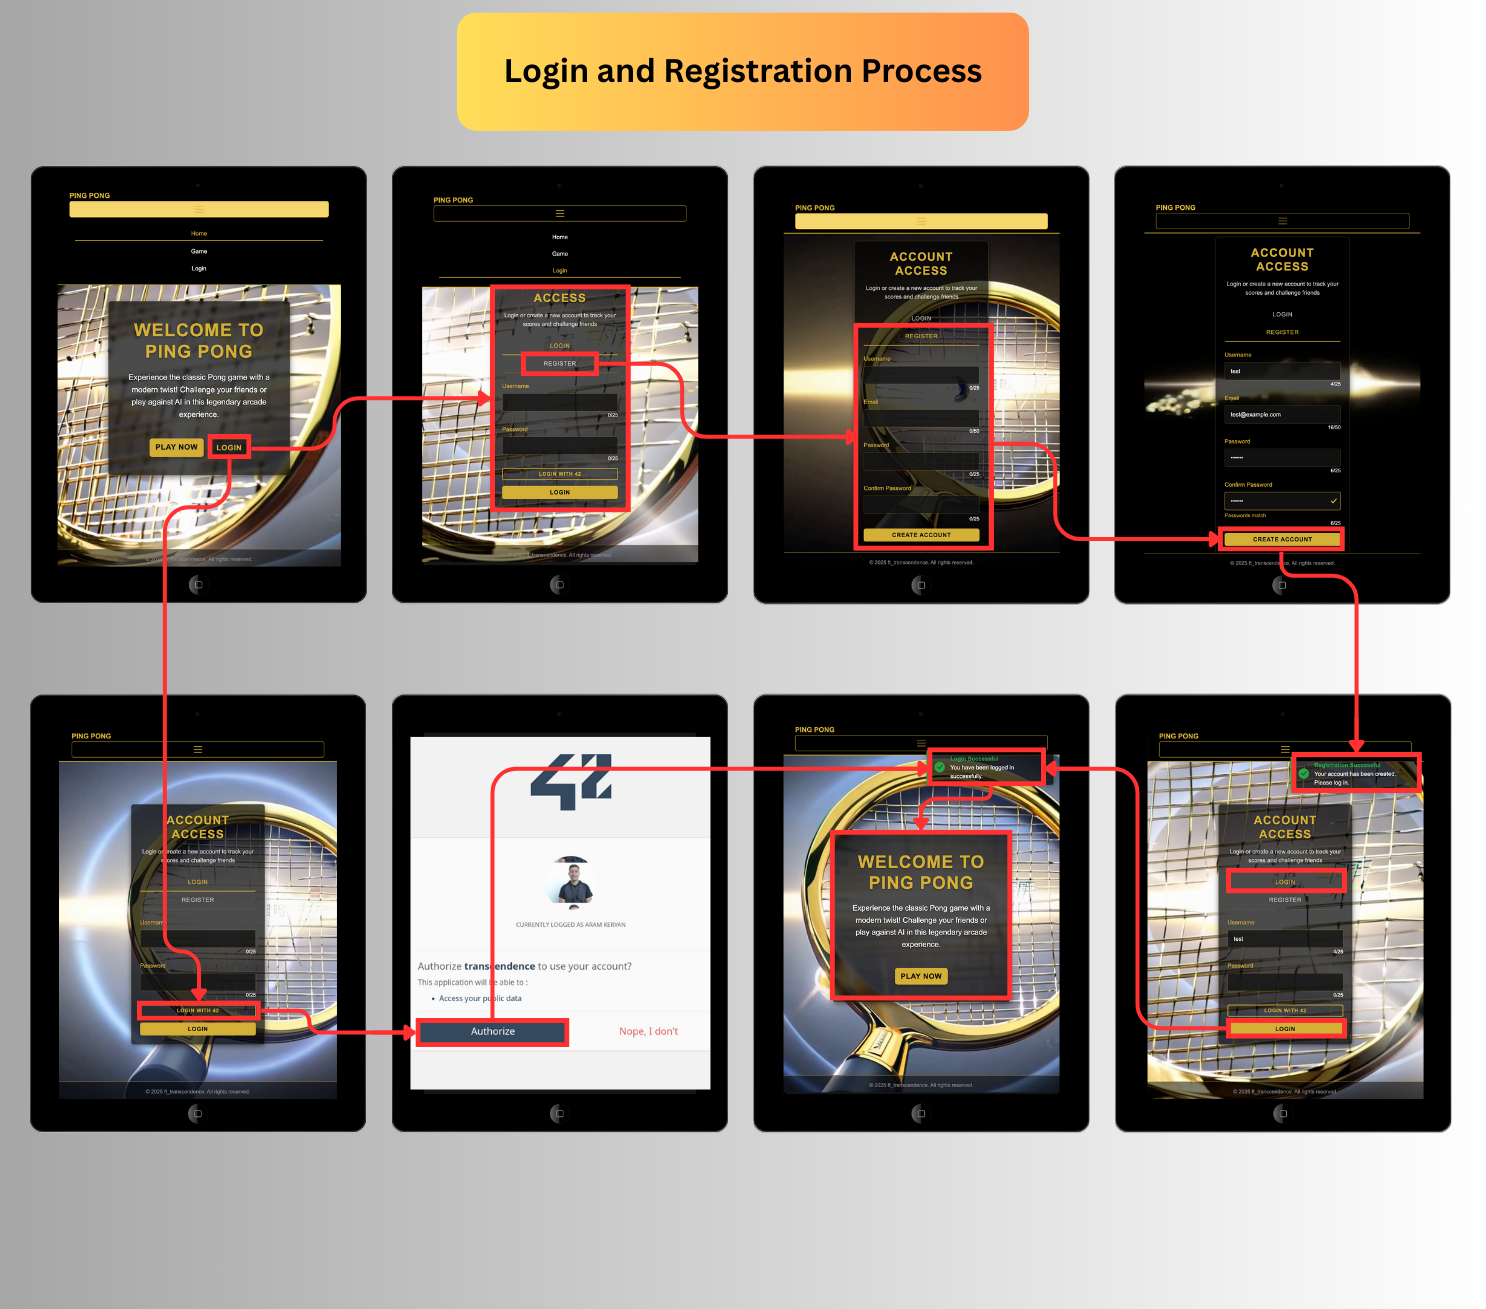
\includegraphics[width=0.9\linewidth]{Figures/images/wireframes/1.png}
    \caption{Authentication and registration wireframe flow showing the complete user journey from initial landing to account creation and login processes}
    \label{fig:wireframe-auth-flow}
\end{figure}

Our authentication flow wireframe demonstrates key HCI principles through:
\begin{itemize}
    \item Sequential and logical progression of interaction steps
    \item Multiple access options (regular login and 42 OAuth) providing user flexibility
    \item Clear input validation patterns with immediate feedback through highlighted error states
    \item Visual hierarchy that guides users through the authentication process with a coherent journey
    \item Contextual hints and feedback at each decision point
\end{itemize}

\subsection{Game Settings and Configuration Flow}

\begin{figure}[H]
    \centering
    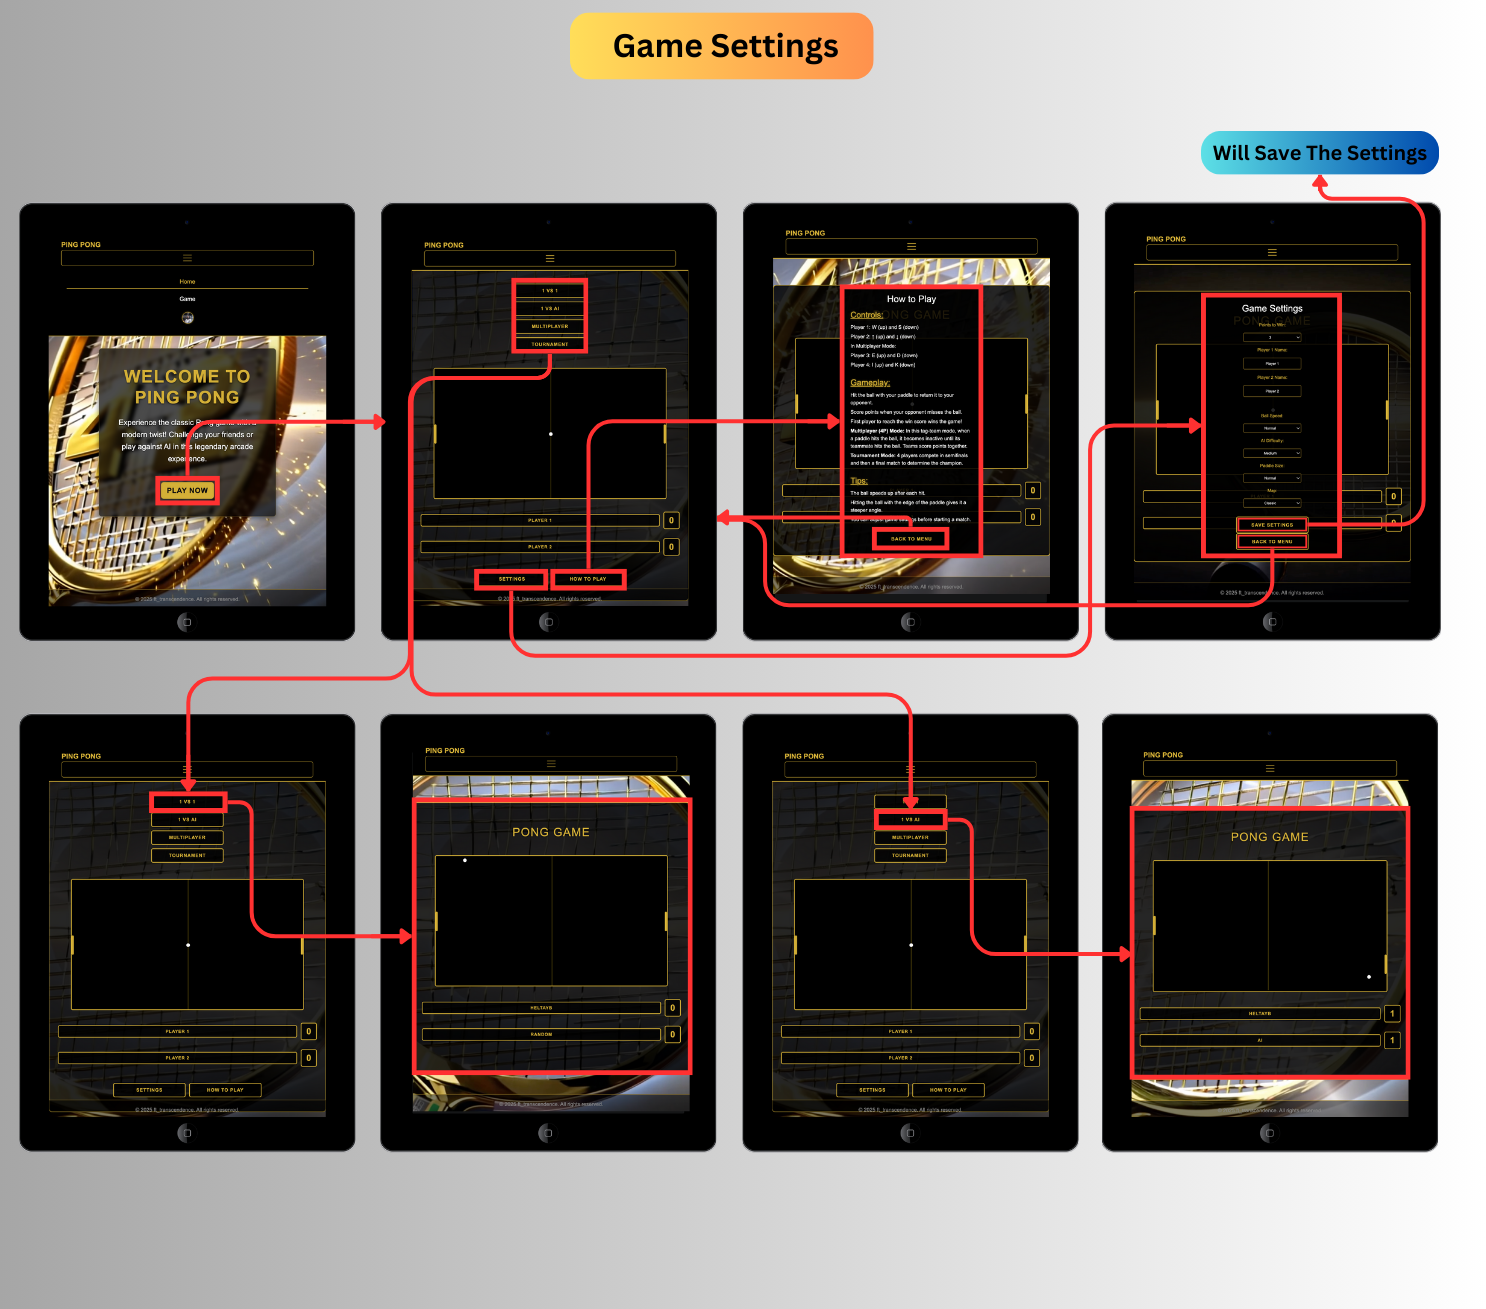
\includegraphics[width=0.9\linewidth]{Figures/images/wireframes/2.png}
    \caption{Game settings wireframe flow showing the progression from home screen to game configuration and play modes}
    \label{fig:wireframe-game-settings}
\end{figure}

The game settings wireframe incorporates UX principles through:
\begin{itemize}
    \item Progressive disclosure - revealing options in a logical sequence
    \item Consistent layout with easily distinguishable game modes and settings
    \item Clear visual feedback for selections and configuration changes
    \item Accessibility considerations through structured navigation paths
    \item Save functionality that acknowledges user preferences and reduces future input needs
\end{itemize}

\subsection{Game Selection and Tournament Mode Flow}

\begin{figure}[H]
    \centering
    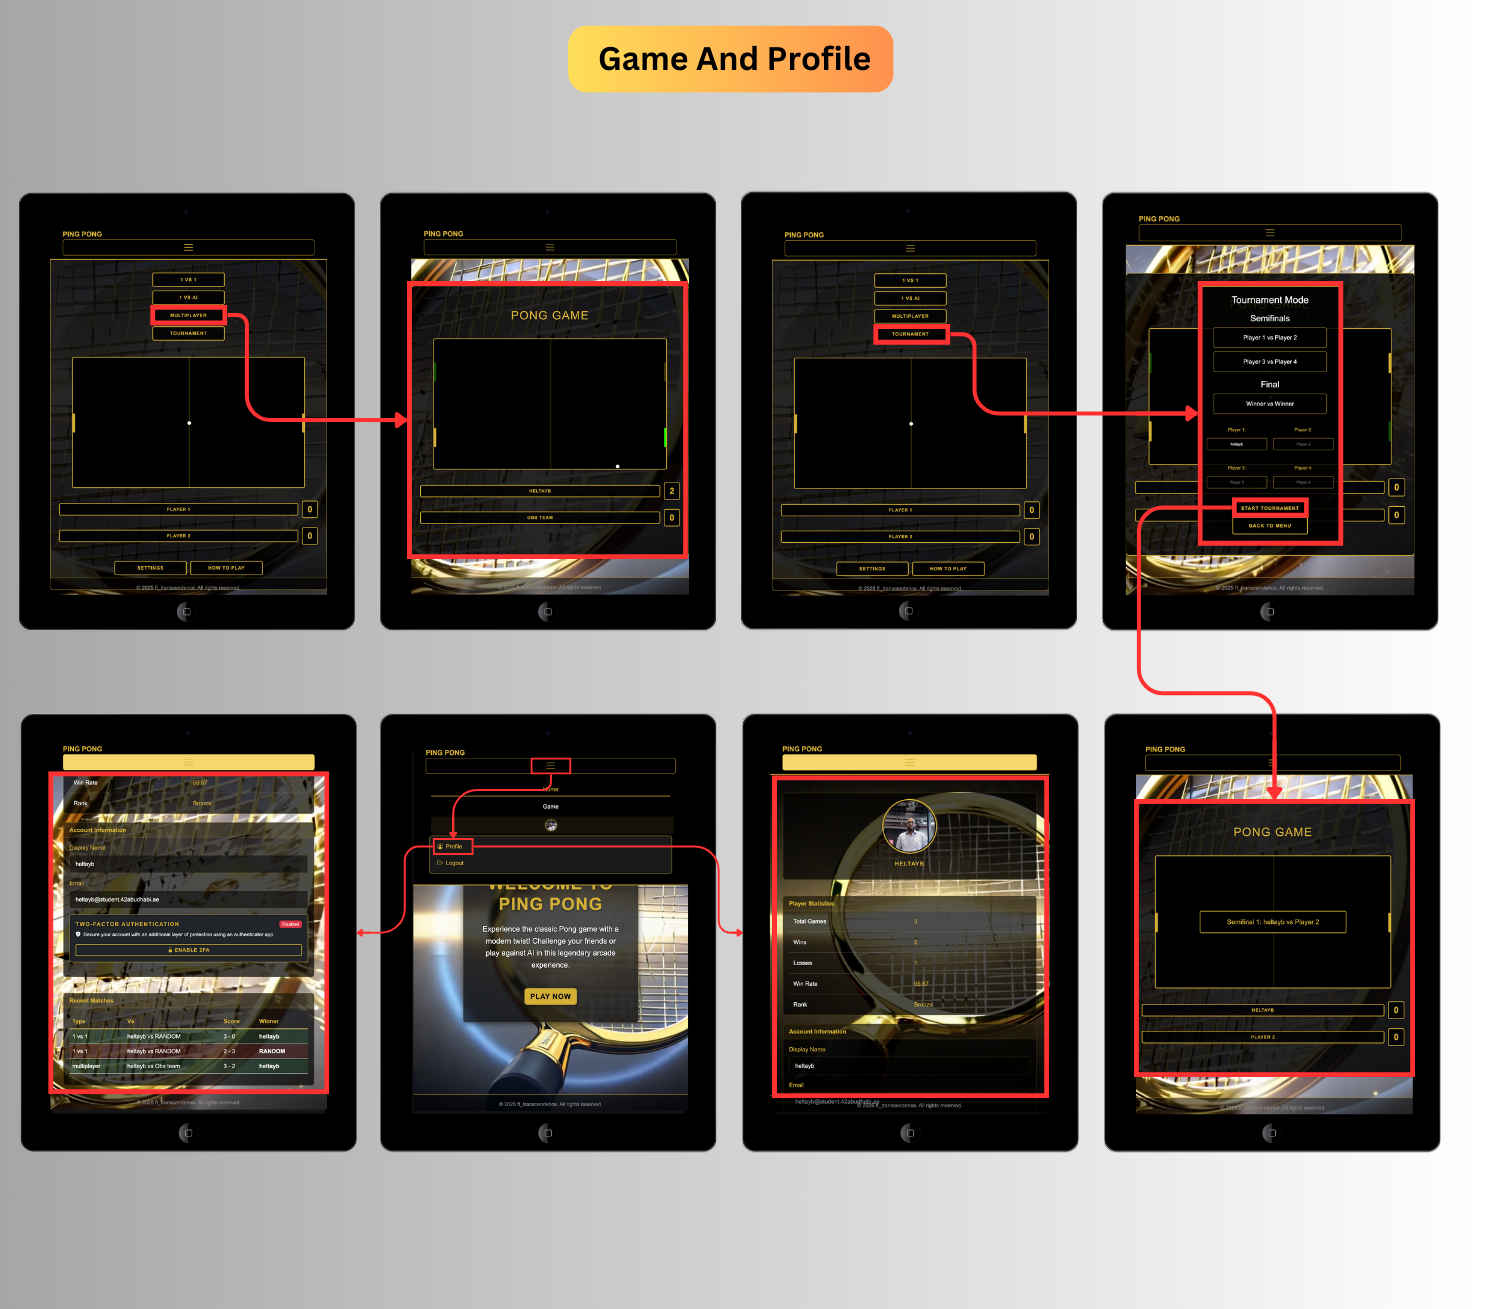
\includegraphics[width=0.9\linewidth]{Figures/images/wireframes/3.png}
    \caption{Game and profile wireframe flow showing tournament structure, gameplay screens, and player statistics integration}
    \label{fig:wireframe-game-tournament}
\end{figure}

The game interface wireframes demonstrate UI design principles through:
\begin{itemize}
    \item Visual representation of tournament brackets enhancing understanding of game progression
    \item Clear player identification and match-up visualization
    \item Consistent game environment across different match types
    \item Seamless integration between game modes and player statistics
    \item Balanced visual layout focusing on gameplay elements and competitive information
\end{itemize}

\subsection{Security Features and Profile Management Flow}

\begin{figure}[H]
    \centering
    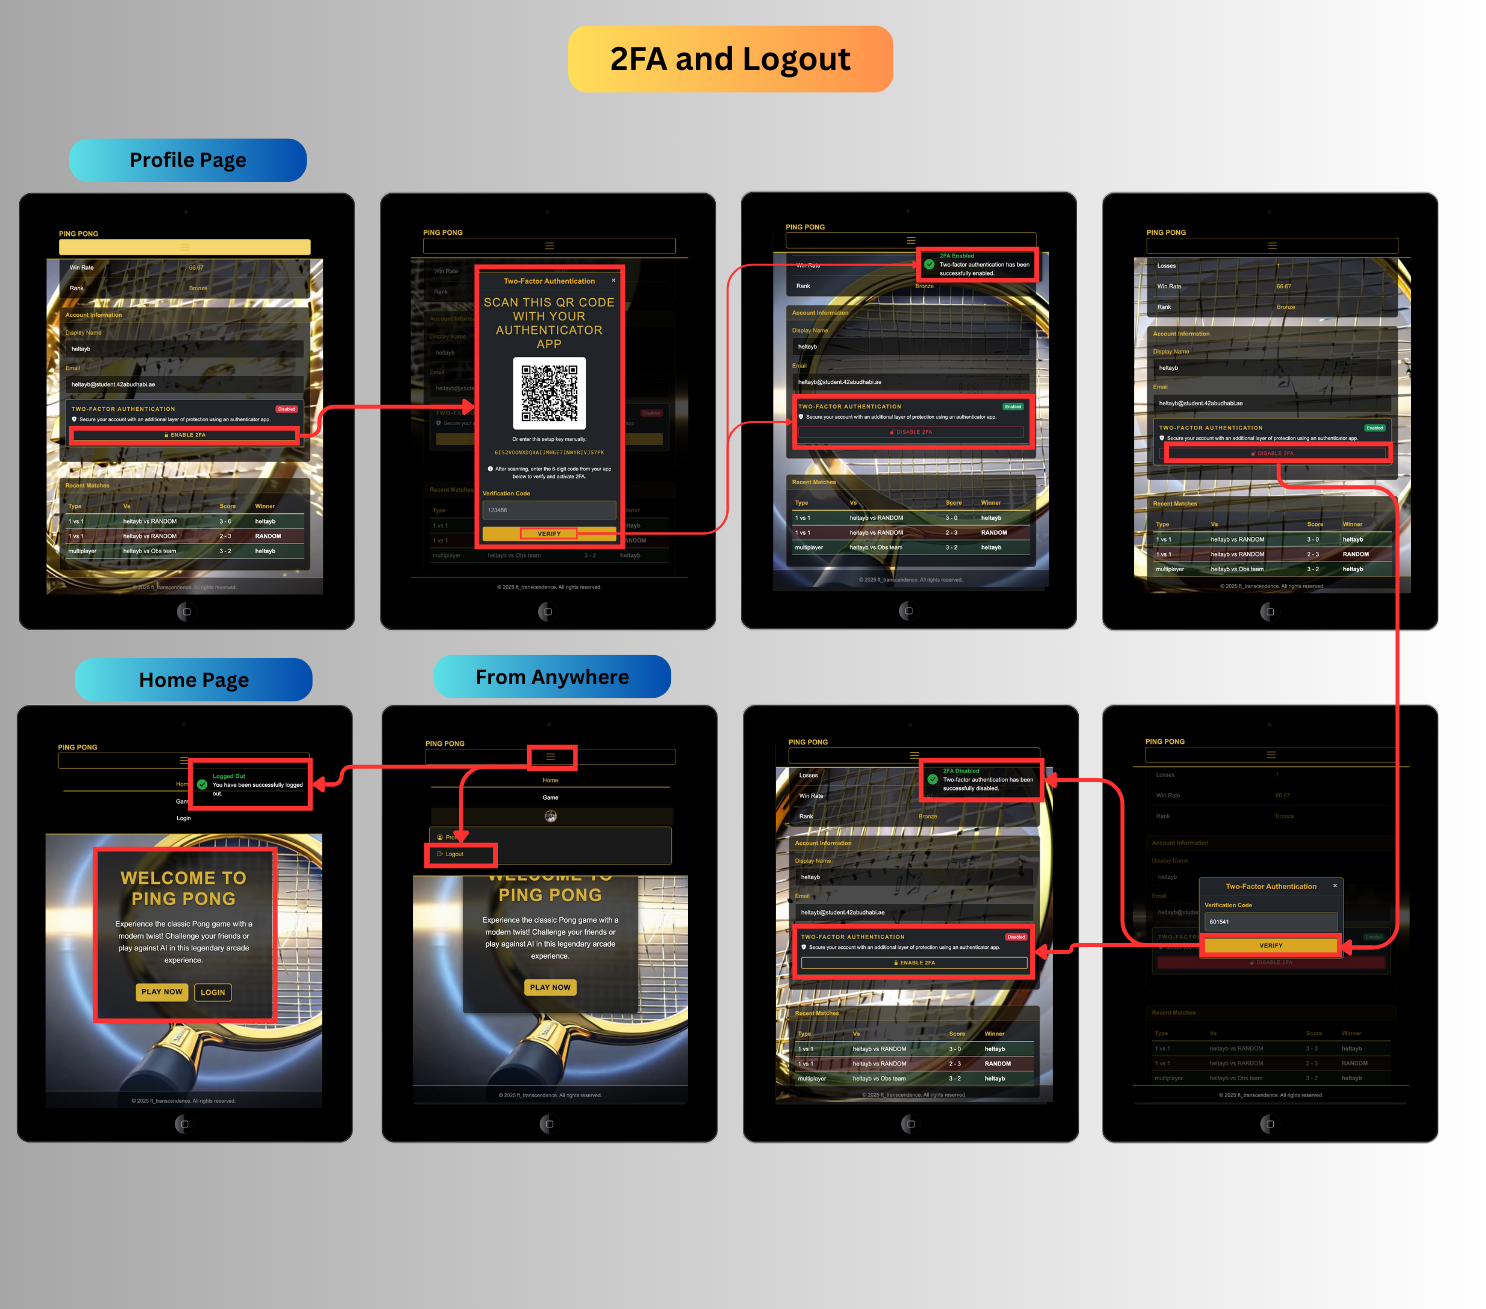
\includegraphics[width=0.9\linewidth]{Figures/images/wireframes/4.png}
    \caption{Two-factor authentication and logout wireframe flow showing security features and session management}
    \label{fig:wireframe-security}
\end{figure}

The security and profile management wireframe demonstrates advanced UX principles through:
\begin{itemize}
    \item Multi-layered security implementation with two-factor authentication
    \item Clear visual cues for secure states and actions
    \item Contextual instruction for security features (QR code scanning)
    \item Consistent feedback for successful actions (login/logout confirmations)
    \item Accessible security features from multiple entry points in the application
\end{itemize}

These comprehensive wireframe flows showcase not just individual screens but the complete user journey through our application. By presenting interconnected screens with navigation paths, we demonstrate our attention to the entire user experience rather than isolated interface components. This approach aligns with modern HCI principles of viewing interfaces as journeys rather than destinations, allowing us to identify potential friction points and optimize the overall user experience.

\section{User Journey Implementation}

Based on the wireframes above, we implemented a comprehensive user interface. The following screens document the complete user journey through the ft\_transcendence application:

\subsection{Beginning the Journey: Registration and Authentication}

When first accessing the application, users are presented with the login page. Here, they have two paths to proceed: they can either log in with existing credentials or register a new account.

\begin{figure}[H]
    \centering
    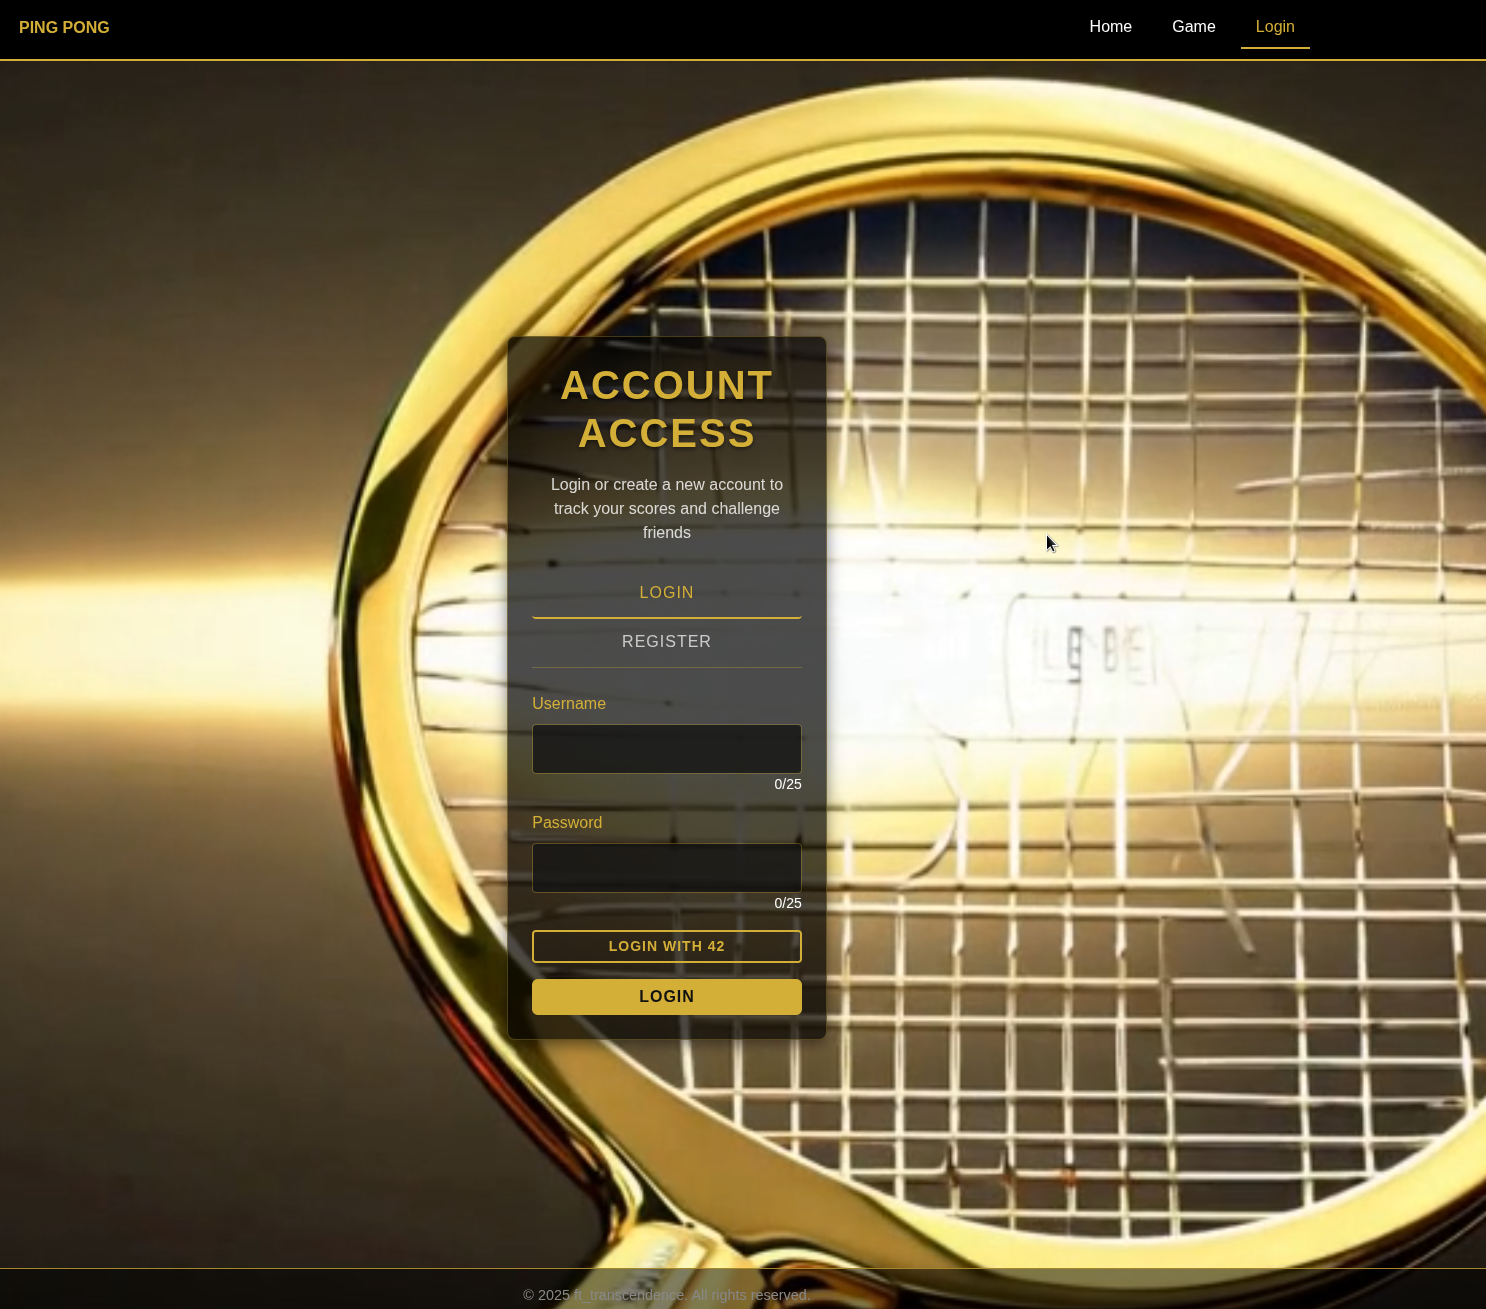
\includegraphics[width=0.7\linewidth]{Figures/images/new_images/LoginPage.png}
    \caption{Login Page.} % Entry point for users with credential-based authentication and 42 OAuth options
    \label{fig:login-page}
\end{figure}

\subsubsection{Path 1: Creating a New Account} For new users, the registration process begins by completing a form with their details. The registration page requires a unique username, valid email address, and secure password.

\begin{figure}[H]
    \centering
    
\includegraphics[width=0.7\linewidth]{Figures/images/new_images/RegistrationPage.png}
    \caption{Registration Page.} % Form for new users to create accounts with validation for username, email and password
    \label{fig:registration-page}
\end{figure}

\begin{figure}[H]
    \centering
    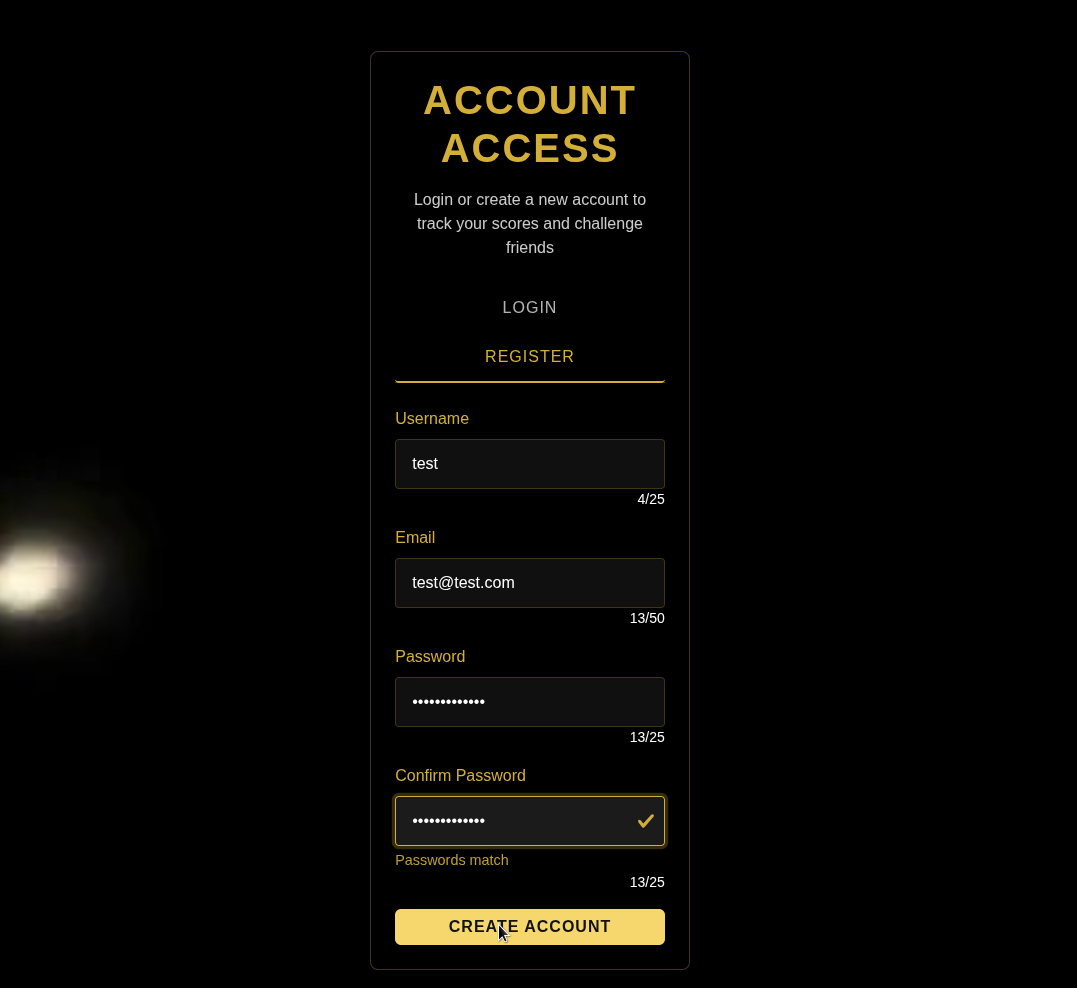
\includegraphics[width=0.7\linewidth]{Figures/images/new_images/RegisteringAccount.png}
    \caption{Account Registration Process.} % Process of filling out registration information
    \label{fig:registering-account}
\end{figure}

During registration, the system validates user input to ensure data quality and security. If a user attempts to submit the form with empty fields, they receive a clear error message:

\begin{figure}[H]
    \centering
    
\includegraphics[width=0.6\linewidth]{Figures/images/new_images/ErrorFillOutAllTheFields.png}
    \caption{Empty Fields Error.} % Validation alert for required form fields
    \label{fig:error-empty-fields-wireframe}
\end{figure}

\begin{figure}[H]
    \centering
    
\includegraphics[width=0.6\linewidth]{Figures/images/new_images/ErrorUserName.png}
    \caption{Username Validation.} % Validation for unique username requirements
    \label{fig:error-username-wireframe}
\end{figure}

The system also validates email format to ensure proper address structure:

\begin{figure}[H]
    \centering
    
\includegraphics[width=0.6\linewidth]{Figures/images/new_images/ErrorEmail.png}
    \caption{Email Validation.} % Email format verification ensuring proper address structure
    \label{fig:error-email-wireframe}
\end{figure}

Passwords must meet security requirements to ensure account protection:

\begin{figure}[H]
    \centering
    
\includegraphics[width=0.6\linewidth]{Figures/images/new_images/ErrorPassword.png}
    \caption{Password Validation.} % Security requirements for creating strong passwords
    \label{fig:error-password-wireframe}
\end{figure}

The system also verifies that password confirmation matches the original entry to prevent typos:

\begin{figure}[H]
    \centering
    
\includegraphics[width=0.6\linewidth]{Figures/images/new_images/ErrorConfirmPassword.png}
    \caption{Password Confirmation.} % Ensuring password entries match during registration
    \label{fig:error-confirm-password-wireframe}
\end{figure}

Upon successful registration, users receive a confirmation message:

\begin{figure}[H]
    \centering
    
\includegraphics[width=0.6\linewidth]{Figures/images/new_images/RegistrationSuccess.png}
    \caption{Registration Success.} % Confirmation of successful account creation
    \label{fig:registration-success-wireframe}
\end{figure}

\subsubsection{Path 2: OAuth with 42 Intra} Alternatively, users with 42 Intra accounts can authenticate through OAuth integration, bypassing the need to create separate credentials:

\begin{figure}[H]
    \centering
    
\includegraphics[width=0.6\linewidth]{Figures/images/new_images/42Login.png}
    \caption{42 Authentication.} % OAuth login option allowing seamless authentication through 42 Intra service
    \label{fig:42-login}
\end{figure}

\begin{figure}[H]
    \centering
    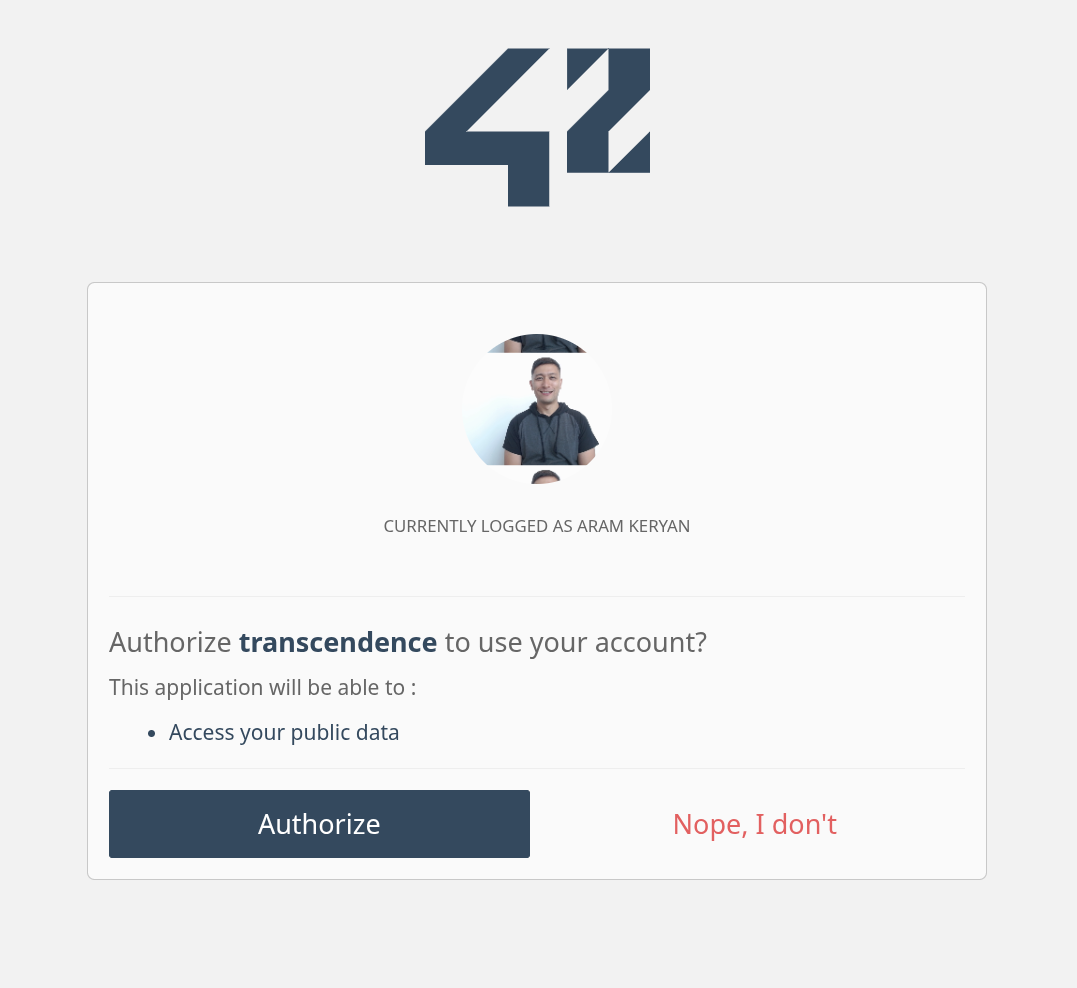
\includegraphics[width=0.6\linewidth]{Figures/images/new_images/42Authentication.png}
    \caption{42 Authentication Process.} % Detailed view of the OAuth authentication process through 42 Intra
    \label{fig:42-auth-process}
\end{figure}

\paragraph{Successful Login} Regardless of the authentication method chosen, upon successful login, users receive a welcome confirmation:

\begin{figure}[H]
    \centering
    
\includegraphics[width=0.6\linewidth]{Figures/images/new_images/LoginSuccessfully.png}
    \caption{Login Success.} % Confirmation of successful authentication
    \label{fig:login-success-wireframe}
\end{figure}

\begin{figure}[H]
    \centering
    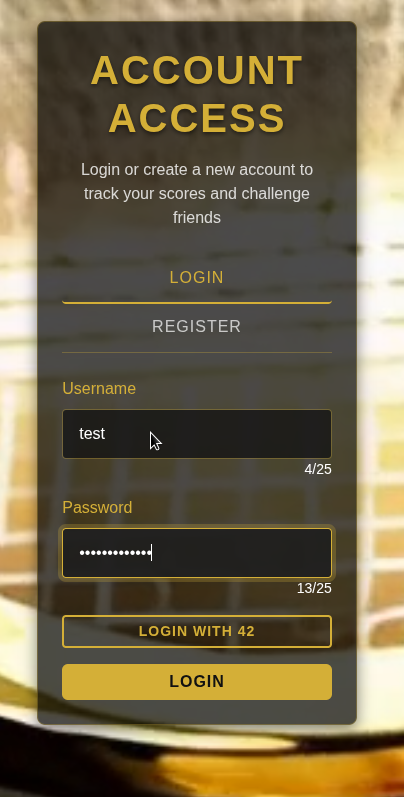
\includegraphics[width=0.6\linewidth]{Figures/images/new_images/LoginWithRegisterdAccount.png}
    \caption{Login With Registered Account.} % Using registered credentials to access the platform
    \label{fig:login-registered-wireframe}
\end{figure}

\subsection{Exploring the Platform: Home Page and Navigation}

After successful login, the user is directed to the home page - the central hub of the application. This modern, clean interface welcomes users and presents the core functionality of the platform.

\begin{figure}[H]
    \centering
    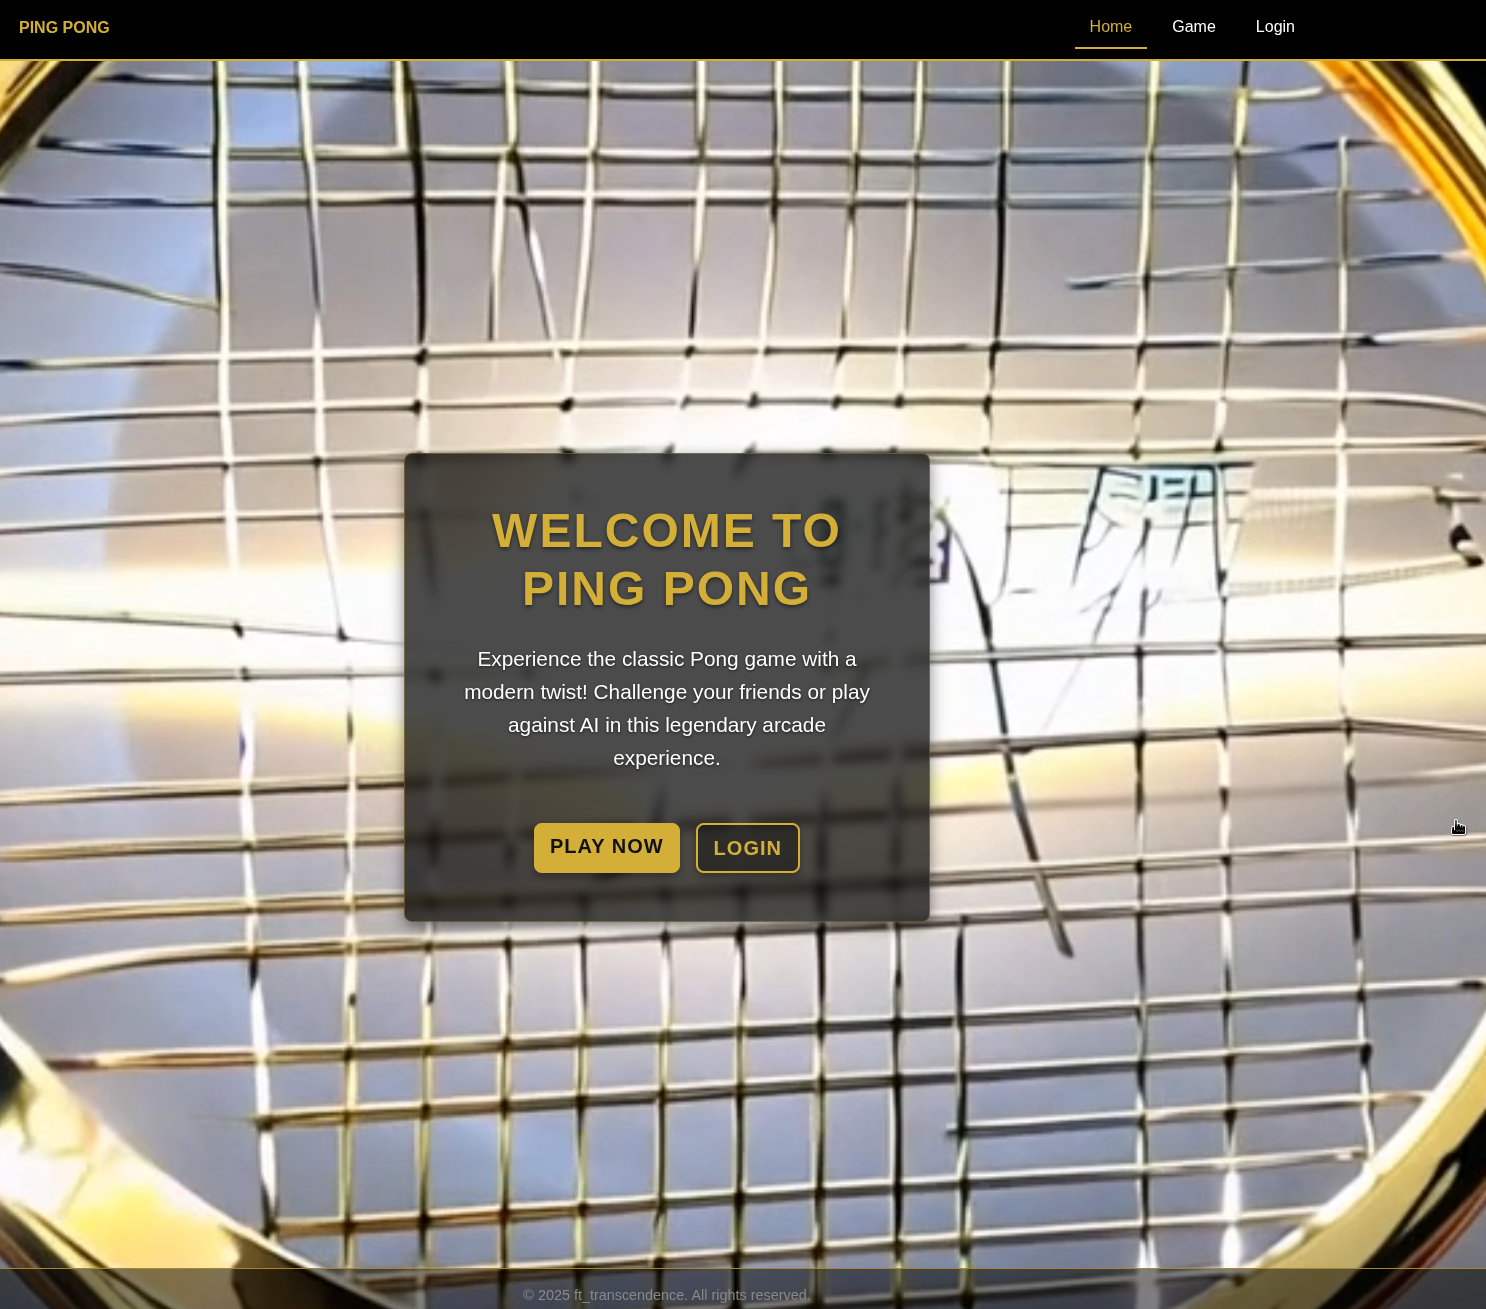
\includegraphics[width=0.7\linewidth]{Figures/images/new_images/HomePage.png}
    \caption{Home Page.} % Dashboard showing navigation options and available game modes after login
    \label{fig:home-page-journey}
\end{figure}

The application features a consistent navigation menu that appears throughout the platform, ensuring users can always access key sections regardless of where they are in the application. This menu provides quick access to game modes, profile management, friends, and settings.

\begin{figure}[H]
    \centering
    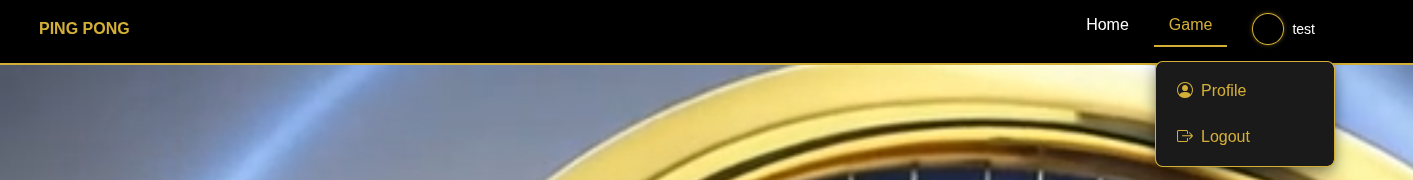
\includegraphics[width=0.65\linewidth]{Figures/images/new_images/MenuBar.png}
    \caption{Menu Bar.} % Navigation providing access to game modes, profile, friends and settings
    \label{fig:menu-bar-journey}
\end{figure}

\subsection{Selecting a Game Mode}

From the home page, users can navigate to the Game page, which serves as the gateway to the core gaming experience. Here, they can select from multiple Pong variants:

\begin{figure}[H]
    \centering
    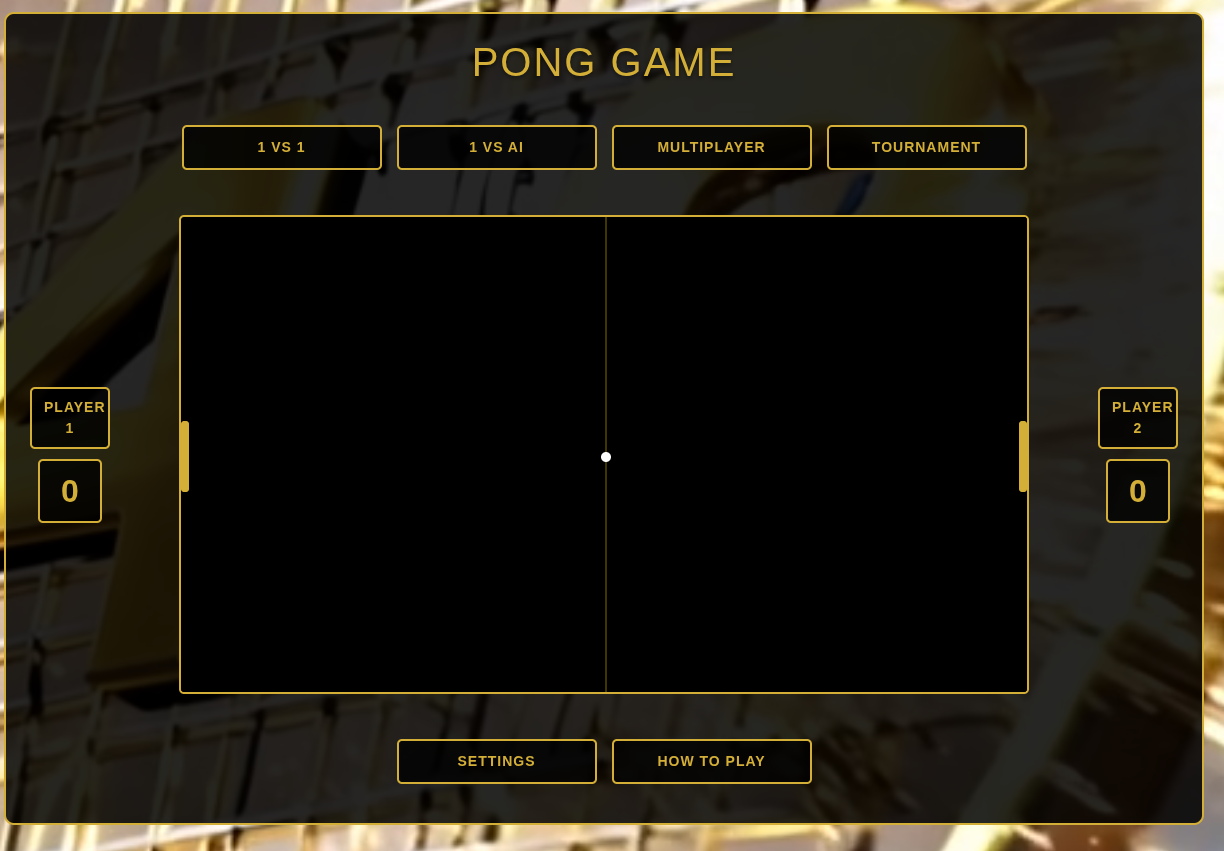
\includegraphics[width=0.7\linewidth]{Figures/images/new_images/GamePage.png}
    \caption{Game Selection.} % Selection hub for different game modes including 1vs1, AI, multiplayer and tournaments
    \label{fig:game-page-journey}
\end{figure}

\subsection{Playing the Game: Exploring Different Game Modes}

Once users have selected a game mode, they enter the actual gameplay experience. The application offers several different ways to enjoy Pong:

\subsubsection{1vs1 Matches} Users can challenge other online players to classic 1vs1 Pong matches. After selecting this mode from the game page, they're taken to the game interface where two human players compete. The screen displays player information, score tracking, and provides intuitive controls (W/S keys for one player, arrow keys for the other).

\begin{figure}[H]
    \centering
    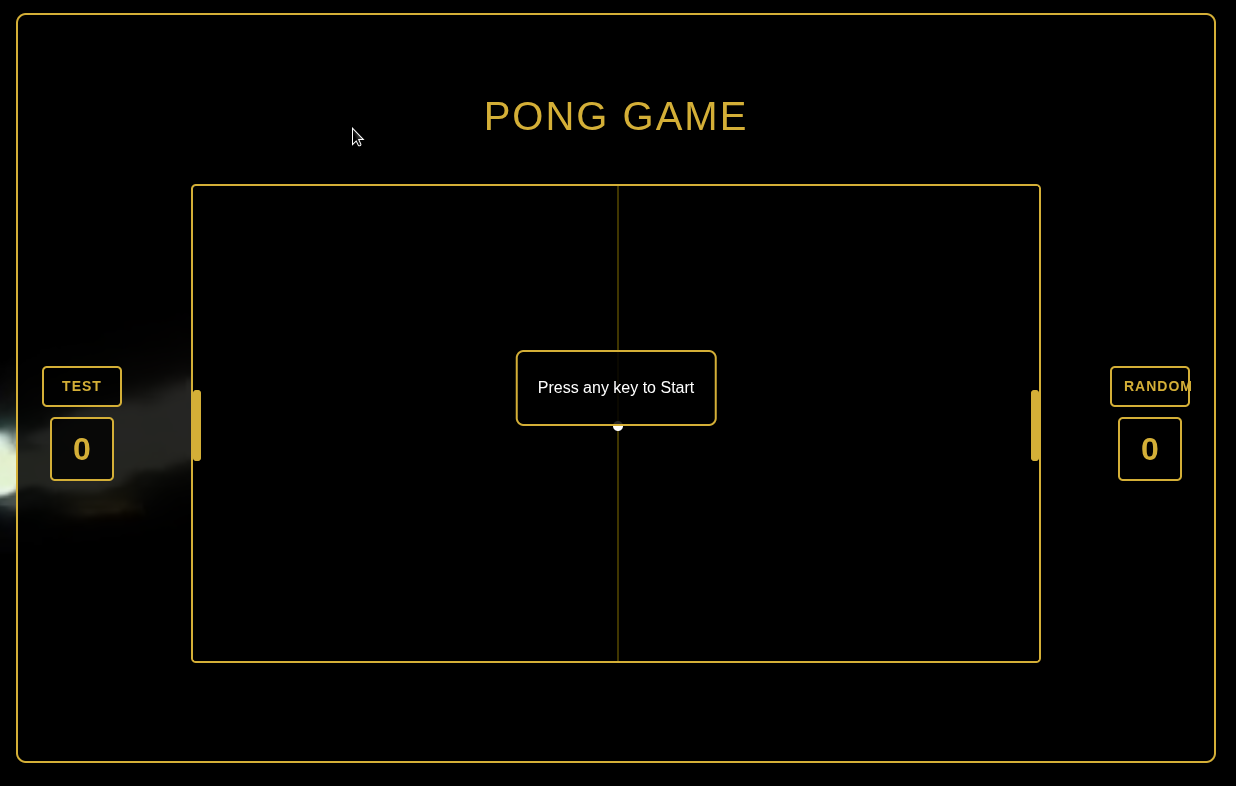
\includegraphics[width=0.65\linewidth]{Figures/images/new_images/Game1vs1.png}
    \caption{1vs1 Game.} % Classic Pong match between two human players with score tracking
    \label{fig:game-1vs1-journey}
\end{figure}

\subsubsection{Practice with AI} For players who want to practice or play solo, the AI opponent mode provides matches against a computer-controlled paddle. This mode maintains the same familiar interface while allowing players to adjust the difficulty level to suit their skill level.

\begin{figure}[H]
    \centering
    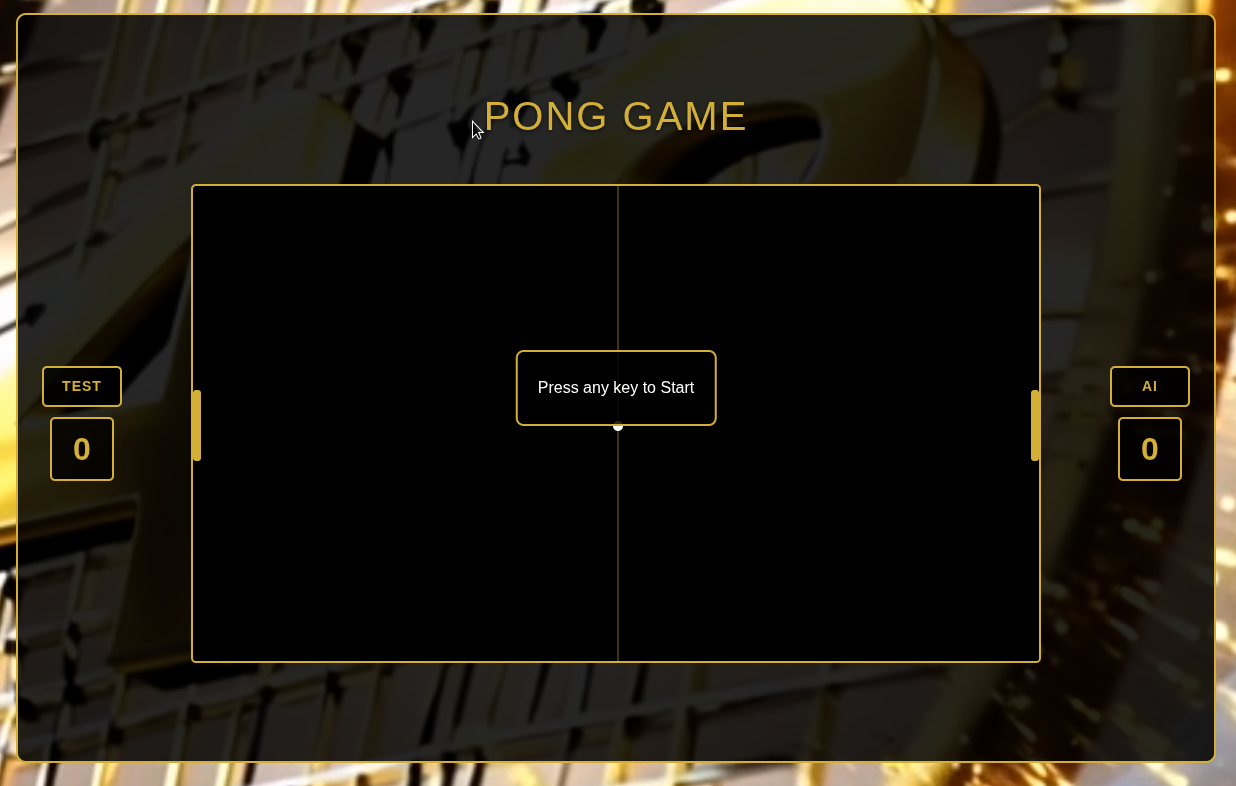
\includegraphics[width=0.65\linewidth]{Figures/images/new_images/Game1vsAI.png}
    \caption{1vs AI Game.} % Practice mode against computer-controlled opponent with adjustable difficulty
    \label{fig:game-1vsai-journey}
\end{figure}

\subsubsection{Local Multiplayer} For social gaming sessions, the multiplayer mode transforms the traditional Pong experience into a dynamic four-player challenge. The interface adapts to place paddles on all four sides of the screen, with each player using different controls for a more social gaming experience.

\begin{figure}[H]
    \centering
    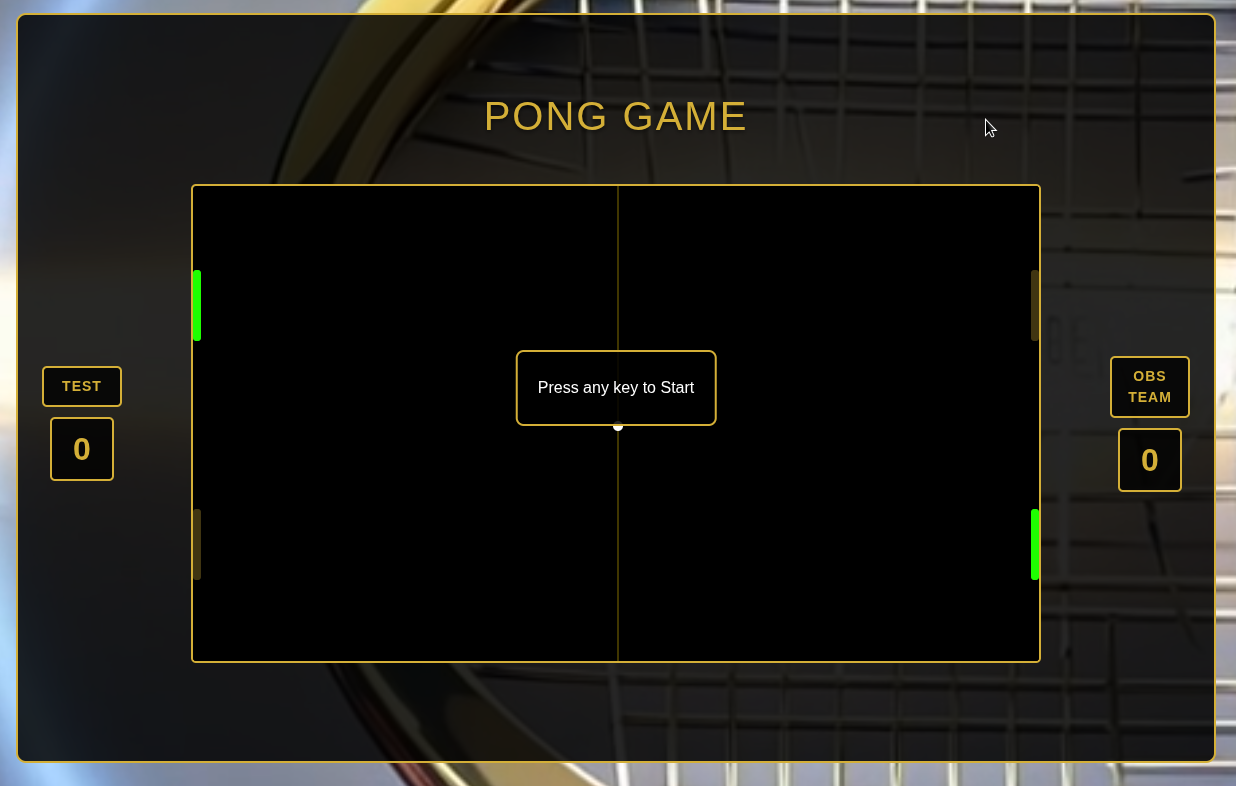
\includegraphics[width=0.65\linewidth]{Figures/images/new_images/GameMultiPlayer.png}
    \caption{Multiplayer Mode.} % Four-player variation with paddles on all sides for local gameplay
    \label{fig:multiplayer-game-journey}
\end{figure}

\subsubsection{Customizing the Experience} Players can personalize their gaming experience through the settings interface. Here they can adjust various parameters including visual preferences, sound options, control layouts, and AI difficulty levels.

\begin{figure}[H]
    \centering
    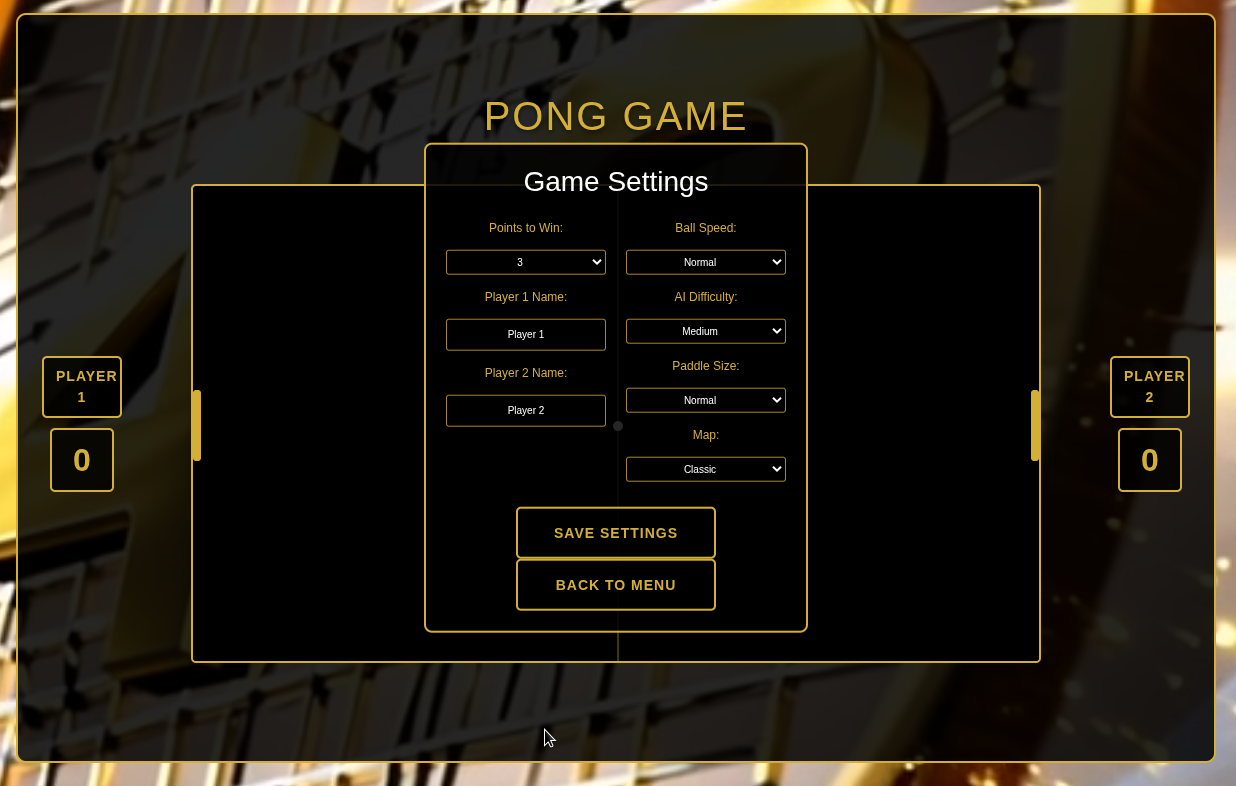
\includegraphics[width=0.65\linewidth]{Figures/images/new_images/GameSettings.png}
    \caption{Game Settings.} % Configuration options for customizing gameplay parameters and preferences
    \label{fig:game-settings-journey}
\end{figure}

\subsubsection{End of Match} When a game concludes, the results screen displays the outcome, final score, and performance statistics. From here, players can choose to play again or return to the main menu.

\begin{figure}[H]
    \centering
    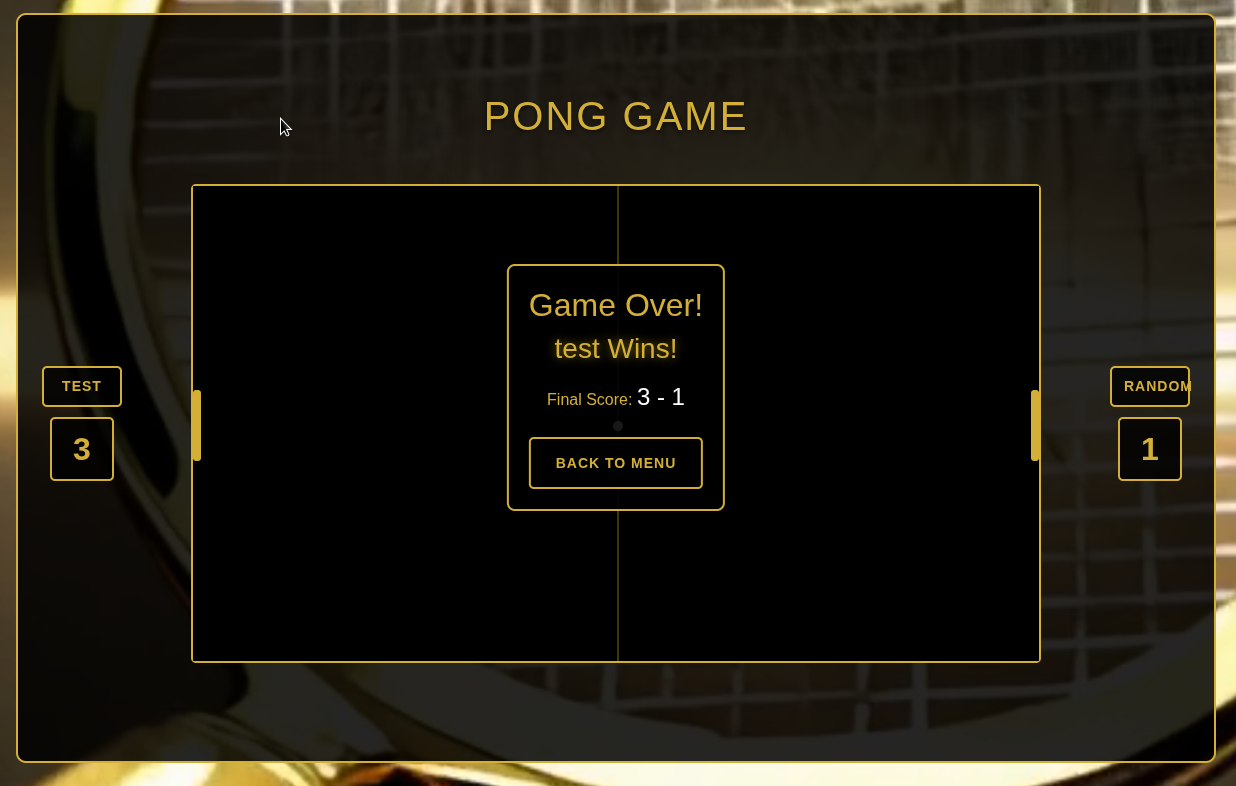
\includegraphics[width=0.65\linewidth]{Figures/images/new_images/GameResult.png}
    \caption{Game Results.} % Match outcome showing final score and player performance statistics
    \label{fig:game-result-journey}
\end{figure}

\subsection{Competing in Tournaments}

For users seeking more structured competition, the tournament mode offers an organized bracket-style experience. After selecting this option from the game page, the user journey continues with tournament participation.

\subsubsection{Joining a Tournament} Users first see the tournament bracket interface that displays all participants and the structure of the competition. Here they can view their position in the bracket, upcoming matches, and track the overall progress of the tournament.

\begin{figure}[H]
    \centering
    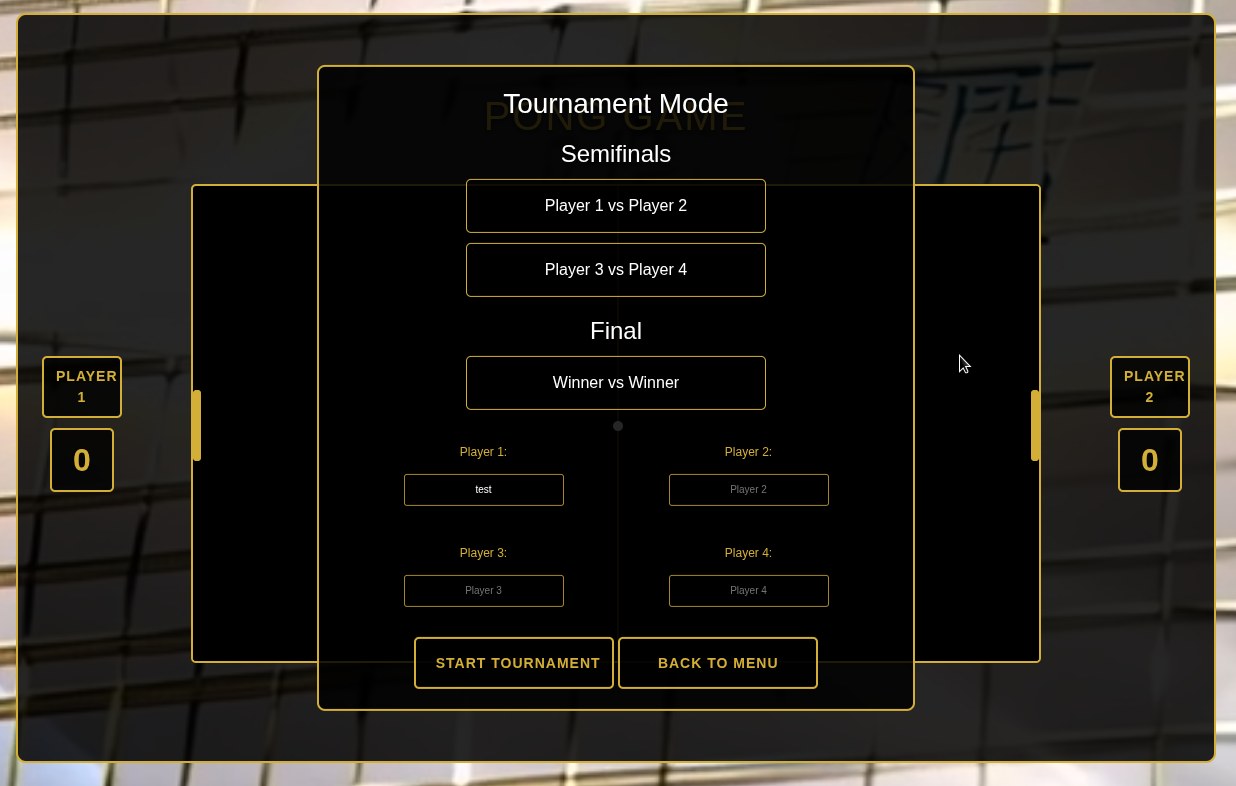
\includegraphics[width=0.65\linewidth]{Figures/images/new_images/GameTournament.png}
    \caption{Tournament Bracket.} % Structured competition showing participating players and bracket progression
    \label{fig:tournament-bracket-journey}
\end{figure}

\subsubsection{Advancing Through Rounds} As users win matches, they progress through the tournament bracket. The semi-final matches maintain the same core gameplay mechanics while highlighting the heightened stakes of the elimination round.

\begin{figure}[H]
    \centering
    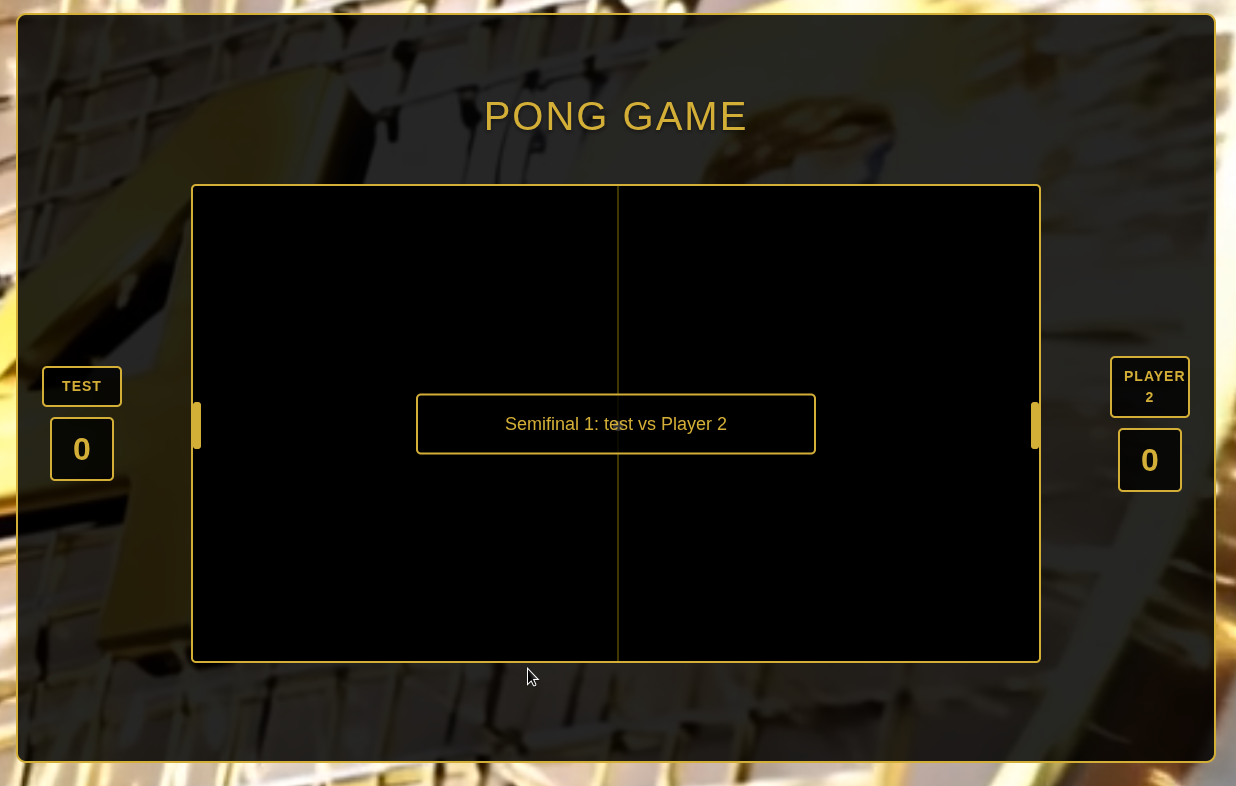
\includegraphics[width=0.65\linewidth]{Figures/images/new_images/GameTournementSemiFinal1.png}
    \caption{Semi-Final Match.} % Tournament elimination round between qualifying players
    \label{fig:tournament-semifinal-journey}
\end{figure}

\subsubsection{Championship} The tournament journey culminates in the final match between the two remaining players. The stakes are highest here, as results from championship matches are not only recorded in the PostgreSQL database but also immutably stored on the Ethereum sidechain, providing a permanent record of achievement.

\begin{figure}[H]
    \centering
    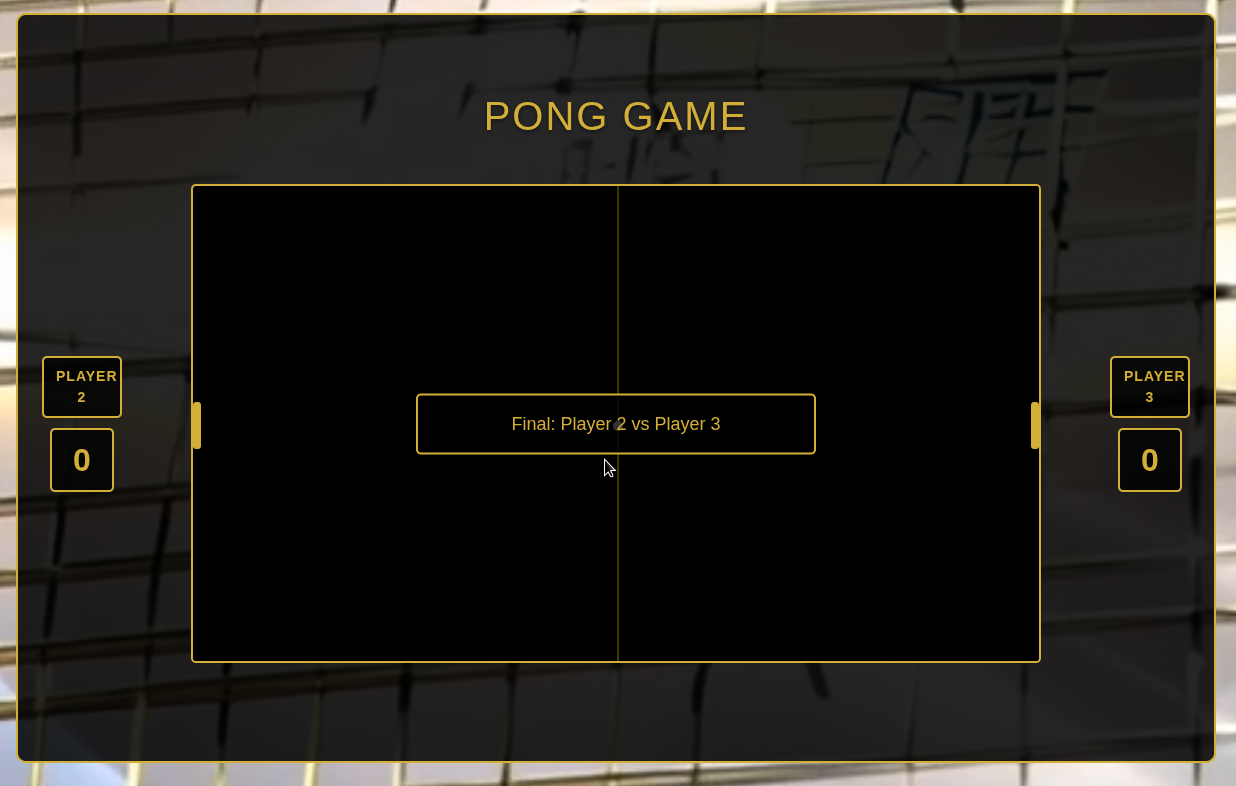
\includegraphics[width=0.65\linewidth]{Figures/images/new_images/GameTournementFinal.png}
    \caption{Tournament Final.} % Championship match with results recorded in database and blockchain
    \label{fig:tournament-final-journey}
\end{figure}

\subsection{Managing Your Profile and Tracking Progress}

Between gaming sessions, users will likely want to review their performance and manage their profile information. The application provides comprehensive profile management tools accessible from the main navigation bar.

\subsubsection{Viewing Your Profile} Users can access their profile page to view their personal statistics, including win/loss ratios, average scores, and ranking information. The profile interface serves as both a personal dashboard and a public-facing representation when viewed by other users.

\begin{figure}[H]
    \centering
    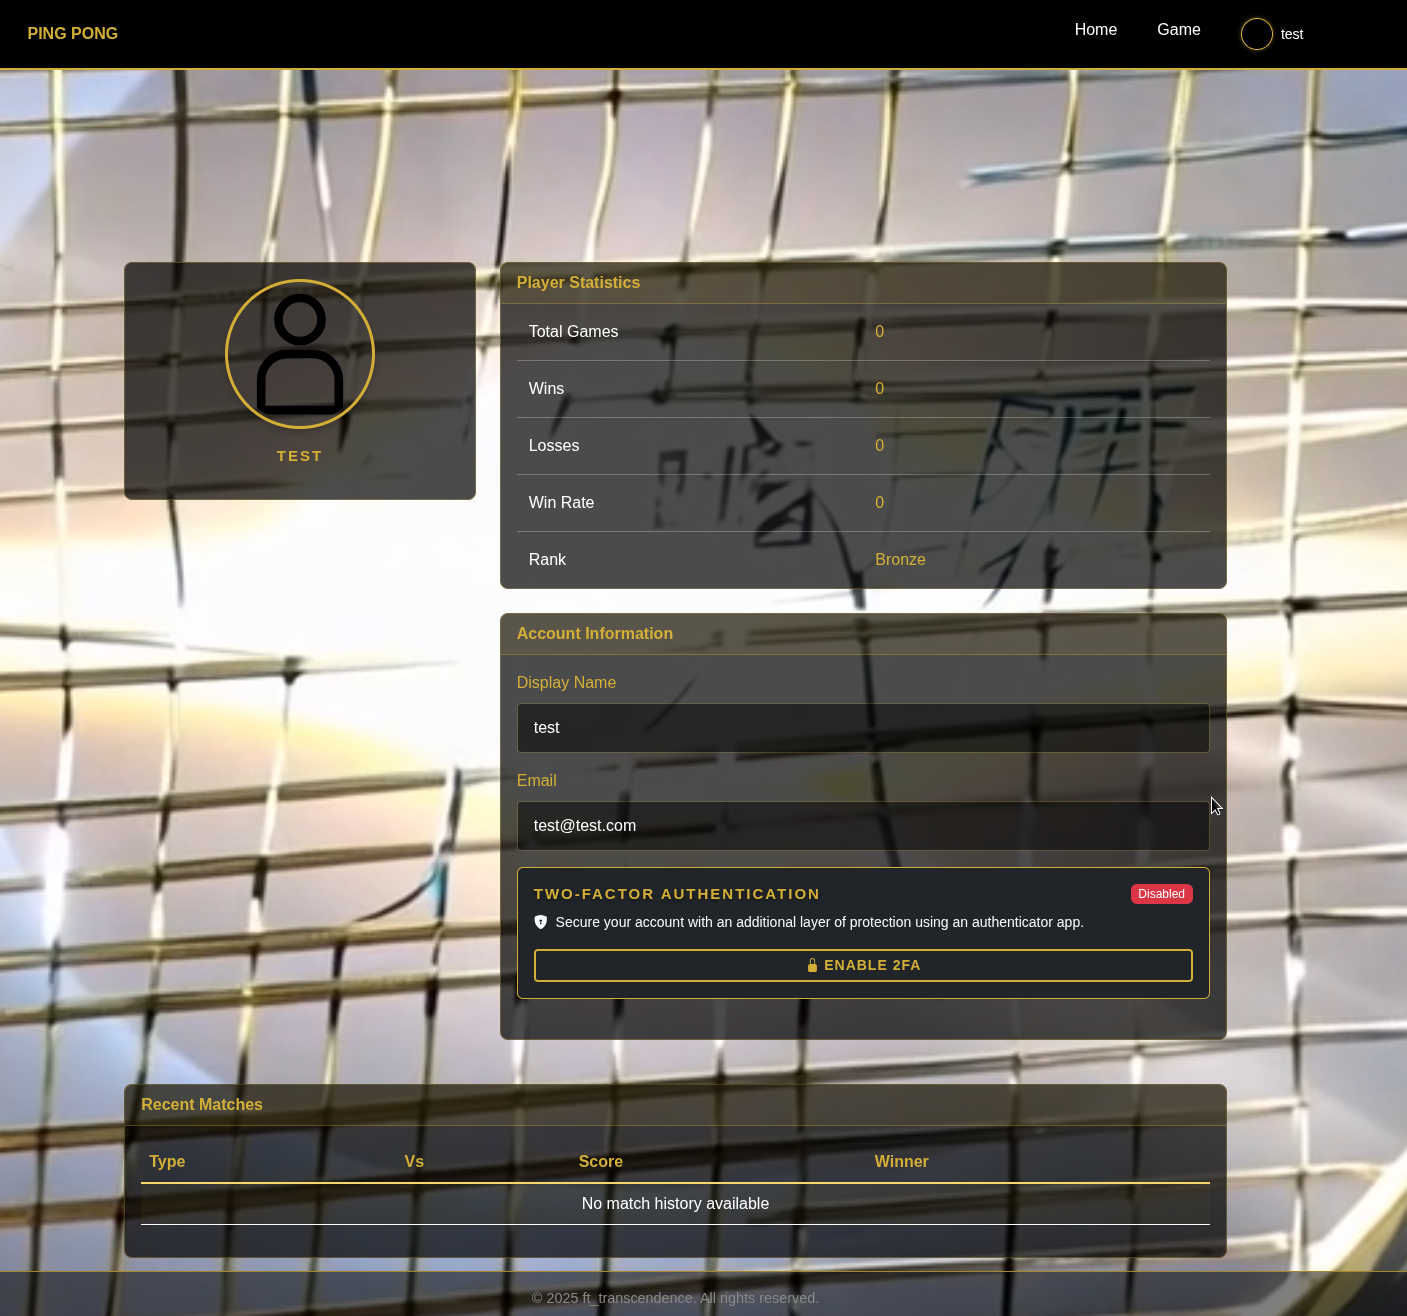
\includegraphics[width=0.65\linewidth]{Figures/images/new_images/ProfilePage.png}
    \caption{User Profile.} % Personal dashboard showing user information and statistics
    \label{fig:profile-page-journey}
\end{figure}

\subsubsection{Reviewing Game History} To help users track their progress and improvement over time, the match history section provides a chronological record of past games. Here users can see their opponents, game outcomes, and performance metrics from previous matches.

\begin{figure}[H]
    \centering
    
\includegraphics[width=0.65\linewidth]{Figures/images/new_images/History.png}
    \caption{Match History.} % Chronological list of past games with outcomes and statistics
    \label{fig:match-history-journey}
\end{figure}

\begin{figure}[H]
    \centering
    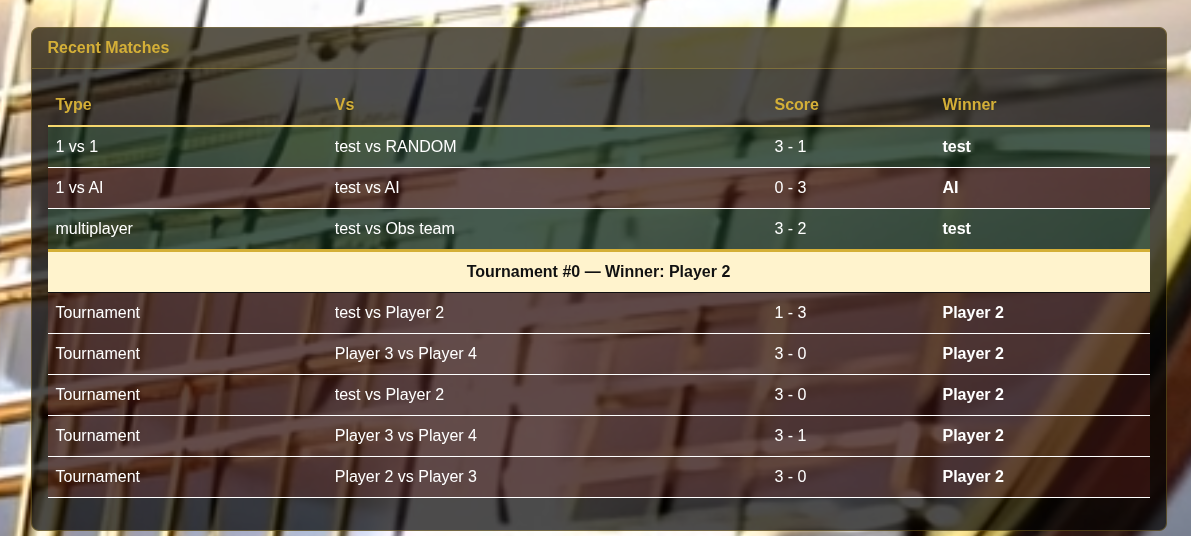
\includegraphics[width=0.65\linewidth]{Figures/images/new_images/RecentMatchesWithData.png}
    \caption{Recent Matches with Data.} % Detailed view of recent match data and statistics
    \label{fig:recent-matches-data-journey}
\end{figure}

\subsubsection{Tracking Performance} Beyond basic profile information, users can access detailed statistics about their gameplay performance. This includes wins and losses, points scored, average game duration, and other performance metrics that help track improvement over time.

\begin{figure}[H]
    \centering
    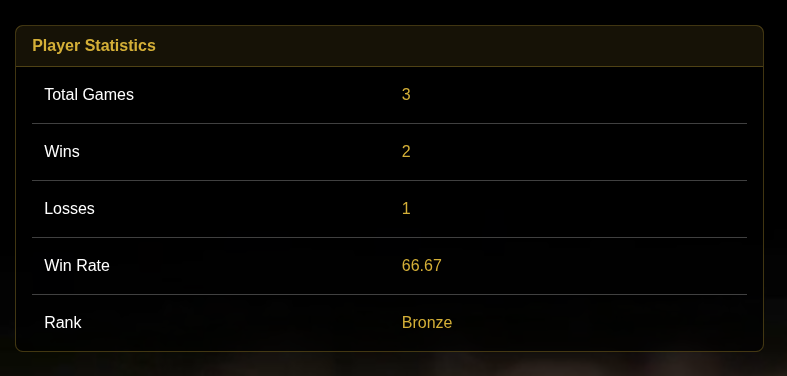
\includegraphics[width=0.65\linewidth]{Figures/images/new_images/PlayerStatisticsWithData.png}
    \caption{Player Statistics.} % Detailed performance metrics and gameplay history
    \label{fig:player-stats-journey}
\end{figure}

\subsection{Managing Your Account and Security}

As users become more engaged with the platform, they may want to personalize their experience further and enhance their account security. The application provides comprehensive account management tools accessible from the navigation menu.

\subsubsection{Account Information} The account settings page displays the user's account details and information. Users can view their account information in this section.

\begin{figure}[H]
    \centering
    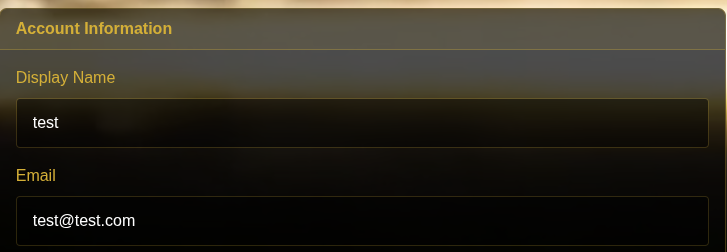
\includegraphics[width=0.65\linewidth]{Figures/images/new_images/AccountInformation.png} % Settings.png not available, using EditProfile as substitute
    \caption{Account Information.} % Page displaying account details
    \label{fig:settings-journey}
\end{figure}

\subsubsection{Enhancing Security} As part of best security practices, the platform offers two-factor authentication (2FA). Users who want to protect their accounts can enable this feature through a guided setup process, linking an authentication app to provide an additional layer of security beyond just a password.

\begin{figure}[H]
    \centering
    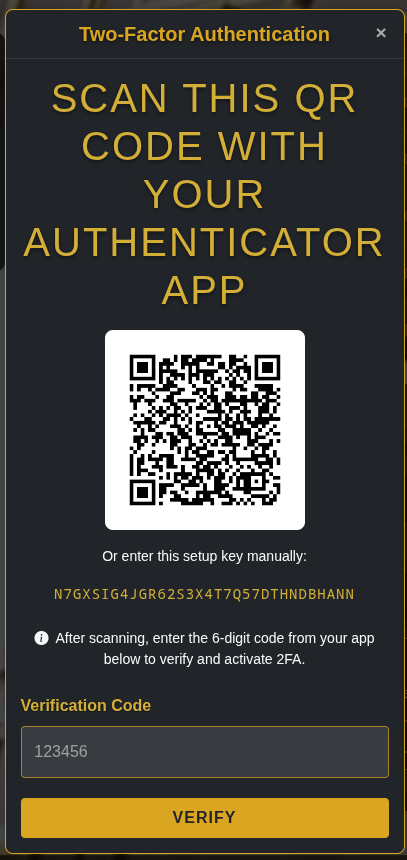
\includegraphics[width=0.4\linewidth]{Figures/images/new_images/Enabling2FA.png}
    \caption{Two-Factor Setup.} % Interface for enabling two-factor authentication security
    \label{fig:2fa-setup-journey}
\end{figure}

\subsubsection{Security Confirmation} After completing the 2FA setup, users receive confirmation that their additional security layer is active. The confirmation screen also provides recovery options to ensure they can regain access if their authentication device is lost or unavailable.

\begin{figure}[H]
    \centering
    
\includegraphics[width=0.65\linewidth]{Figures/images/new_images/2FASuccessfullyEnabled.png}
    \caption{Security Confirmation.} % Successful setup of two-factor authentication
    \label{fig:2fa-confirmation-journey}
\end{figure}

\subsubsection{Two-Factor Authentication Status} Users can verify the status of their two-factor authentication. The platform clearly indicates whether 2FA is currently enabled or disabled for their account.

\begin{figure}[H]
    \centering
    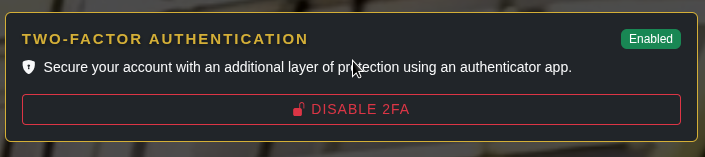
\includegraphics[width=0.65\linewidth]{Figures/images/new_images/2FAEnabled.png}
    \caption{2FA Enabled Status.} % Visual indication that two-factor authentication is active
    \label{fig:2fa-enabled-journey}
\end{figure}

\begin{figure}[H]
    \centering
    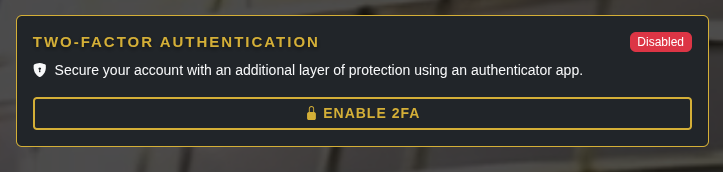
\includegraphics[width=0.65\linewidth]{Figures/images/new_images/2FADisabled.png}
    \caption{2FA Disabled Status.} % Visual indication that two-factor authentication is inactive
    \label{fig:2fa-disabled-journey}
\end{figure}

\subsection{Ending Your Session: Logout}

When users are ready to end their session, the application provides a straightforward logout process.

\subsubsection{Logout Process} Users can access the logout option from the navigation menu. Upon selecting logout, the system securely terminates their session and displays a confirmation message.

\begin{figure}[H]
    \centering
    
\includegraphics[width=0.65\linewidth]{Figures/images/new_images/LogoutSuccessfully.png}
    \caption{Logout Confirmation.} % Notification of successful session termination
    \label{fig:logout-confirmation-journey}
\end{figure}

\subsubsection{Journey Completion} After logout, users are redirected to the login page, completing the full user journey cycle. This clear boundary between sessions helps maintain security while providing an obvious re-entry point for the next visit.

\subsection{Form Validation Throughout the Journey}

Throughout the user journey, the application implements comprehensive form validation to ensure data integrity and provide clear feedback:

\subsubsection{Empty Field Validation} When forms are submitted with missing information, the system displays targeted validation messages.

\begin{figure}[H]
    \centering
    
\includegraphics[width=0.65\linewidth]{Figures/images/new_images/ErrorFillOutAllTheFields.png}
    \caption{Empty Fields Alert.} % Validation message for incomplete form submission
    \label{fig:error-empty-fields-journey}
\end{figure}

\subsubsection{Email Format Validation} The system verifies that email addresses conform to proper formatting standards.

\begin{figure}[H]
    \centering
    
\includegraphics[width=0.65\linewidth]{Figures/images/new_images/ErrorEmail.png}
    \caption{Email Format Alert.} % Validation message for incorrectly formatted email address
    \label{fig:error-email-journey}
\end{figure}

\subsubsection{Password Requirements} To enhance security, the application enforces password strength policies.

\begin{figure}[H]
    \centering
    
\includegraphics[width=0.65\linewidth]{Figures/images/new_images/ErrorPassword.png}
    \caption{Password Strength Alert.} % Validation message for password that doesn't meet security requirements
    \label{fig:error-password-journey}
\end{figure}

\subsubsection{Password Matching} The system ensures that password confirmation fields match the initially entered password.

\begin{figure}[H]
    \centering
    
\includegraphics[width=0.65\linewidth]{Figures/images/new_images/ErrorConfirmPassword.png}
    \caption{Password Mismatch Alert.} % Error message when password and confirmation don't match
    \label{fig:error-confirm-password-journey}
\end{figure}

\subsection{Journey Conclusion}

The wireframes presented in this chapter illustrate the complete user journey through the ft\_transcendence application, from initial registration to gameplay and eventual logout. This cohesive flow demonstrates how the various screens and interfaces work together to create a seamless user experience that is both intuitive and engaging.

The journey begins with authentication, progresses through exploration of the platform's features and gameplay, allows for social interaction and profile management, provides security options, and concludes with a clear session ending. Throughout this journey, users encounter consistent navigation patterns, clear feedback mechanisms, and intuitive interfaces that collectively deliver a polished and professional gaming experience.



\chapter{Detailed System Design and Implementation}
\label{ch:implementation}

This chapter delves into the specific implementation details of the core components of the \textbf{ft\_transcendence} application, expanding on the architectural overview provided previously. It covers the backend logic, frontend structure, data persistence mechanisms, real-time communication, and the containerization strategy.

\section{Backend Implementation (Django)}
\label{sec:backend_impl}
The backend is built using the Django framework (version 5), leveraging its robust features for web development and the Django Rest Framework (DRF) for creating the RESTful API.

\subsection{Project Structure}
The Django project follows a standard layout, organized into distinct apps for modularity:
\begin{itemize}
    \item \texttt{users}: Handles user registration, authentication (native credentials, 42 OAuth), and basic profile information.
    \item \texttt{game}: Contains the logic for Pong gameplay, including game state management, rules enforcement, and matchmaking (for 1v1 online).
    \item \texttt{tournaments}: Manages the creation, progression, and recording of tournament brackets.
\end{itemize}

\subsection{API Design (DRF)}
The API provides endpoints for frontend interaction. DRF's ViewSets and Serializers are used to handle data validation, database interaction, and JSON response generation. Key endpoints likely include:
\begin{itemize}
    \item User authentication and registration.
    \item User profile information access.
    \item Game initiation and state updates.
    \item Tournament creation and status retrieval.
    \item Match history access.
\end{itemize}

\subsection{Authentication and Authorization}
Security is managed through multiple layers:
\begin{itemize}
    \item \textbf{Native Credentials:} Standard username/password login.
    \item \textbf{42 OAuth:} Integration with the 42 Intra's OAuth2 system for seamless login for 42 students.
    \item \textbf{JWT (JSON Web Tokens):} Simple-JWT library is used to issue JWTs stored in secure HTTP-only cookies upon successful login, authenticating subsequent API requests.
    \item \textbf{2FA (TOTP):} Optional Time-based One-Time Password (TOTP) using \texttt{django-otp} provides an additional security layer.
\end{itemize}

\section{Frontend Implementation (Vanilla JS)}
\label{sec:frontend_impl}
The frontend is a Single Page Application (SPA) built entirely with vanilla JavaScript (ES6+), HTML5, and styled with Bootstrap 5. This approach avoids reliance on heavy frontend frameworks.

\subsection{SPA Architecture}
JavaScript manages routing (likely using the History API or hash-based routing) to dynamically load content and views without full page reloads. State management might be handled through simple JavaScript objects or potentially a lightweight custom solution.

\subsection{Rendering}
\begin{itemize}
    \item \textbf{Game Interface:} The core Pong gameplay (paddles, ball, score) is rendered dynamically on an HTML5 \texttt{<canvas>} element, providing fine-grained control over animations and interactions.
    \item \textbf{UI Elements:} Other interface components (dashboard, login forms, profile page, menus) are built using standard HTML elements manipulated via the Document Object Model (DOM) by JavaScript. Bootstrap provides styling and layout components.
\end{itemize}

\subsection{API Interaction}
The frontend communicates with the Django backend via asynchronous JavaScript (e.g., using the \texttt{fetch} API) to send requests to the RESTful API endpoints and receive data in JSON format. Real-time updates (discussed below) are handled separately.

\section{Database Implementation}
\label{sec:database_impl}
Data persistence relies on two distinct systems:

\subsection{PostgreSQL}
A PostgreSQL (version 15) relational database serves as the primary datastore for user accounts, basic profile information, game settings, and detailed match history. Django's ORM (Object-Relational Mapper) facilitates interaction with the database.

\subsection{Ethereum Sidechain}
For tournament results, an Ethereum-compatible sidechain (potentially using Proof of Authority) is employed to ensure immutable and verifiable record-keeping. The Django backend interacts with a deployed smart contract via the \texttt{Web3.py} library to record the winners and potentially other key tournament data.


\section{DevOps and Containerization (Docker)}
\label{sec:devops_impl}
The entire application stack is containerized using Docker and orchestrated with Docker Compose, facilitating consistent development, testing, and deployment environments.

The \texttt{docker-compose.yml} file defines the services:
\begin{itemize}
    \item \textbf{Backend:} Runs the Django application (likely using Gunicorn or Uvicorn).
    \item \textbf{Frontend/Nginx:} An Nginx container serves the static frontend files (HTML, CSS, JS) and acts as a reverse proxy for the Django backend. It also handles TLS termination for HTTPS.
    \item \textbf{Database:} A PostgreSQL container manages the relational data.
    \item \textbf{ELK Stack:} Separate containers for Elasticsearch and Kibana handle centralized logging and monitoring.
\end{itemize}
Makefiles are likely used to streamline common Docker operations like building images, starting/stopping containers, and running management commands.

\chapter{Testing and Evaluation}
\label{ch:testing}

Ensuring the quality, reliability, and security of the \textbf{ft\_transcendence} application is paramount. This chapter details the testing strategies employed throughout the development lifecycle and provides an evaluation of the project against its initial objectives.

\section{Testing Strategy}
\label{sec:testing_strategy}
A multi-layered testing approach was adopted to verify different aspects of the application:
\begin{itemize}
    \item \textbf{Unit Testing:} Focused on verifying the correctness of individual components (functions, classes) in isolation.
    \item \textbf{Integration Testing:} Examined the interactions between different modules and services (e.g., backend API with database, frontend with backend).
    \item \textbf{End-to-End (E2E) Testing:} Validated complete user workflows from the user's perspective.
    \item \textbf{Security Testing:} Assessed the application's resilience against common web vulnerabilities and ensured security features function correctly.
    \item \textbf{Usability and Accessibility Testing:} Evaluated the user-friendliness of the interface and the effectiveness of accessibility features.
\end{itemize}

\section{Unit Testing}
\label{sec:unit_testing}
Unit tests formed the foundation of the testing pyramid, providing rapid feedback on code changes.
\begin{itemize}
    \item \textbf{Backend (Django):} Django's built-in testing framework was likely utilized to write tests for models (database logic), views (API endpoint logic), serializers (data validation), and utility functions. Mocking was used where necessary to isolate units from external dependencies like the database or external APIs (e.g., 42 OAuth during testing).
    \item \textbf{Frontend (Vanilla JS):} Unit testing vanilla JavaScript can be challenging. While specific tools might not have been mandated, critical utility functions or logic components might have been tested using a framework like Jest or through manual verification during development.
\end{itemize}

\section{Integration Testing}
\label{sec:integration_testing}
Integration tests focused on verifying the correct communication and data flow between different parts of the system.
\begin{itemize}
    \item \textbf{API Level:} Tests were conducted to ensure that frontend requests to the Django REST Framework API endpoints resulted in the correct backend actions (e.g., database updates) and generated the expected responses (status codes, data formats).
    \item \textbf{Database Interaction:} Verified that the Django ORM correctly interacted with the PostgreSQL database, ensuring data integrity and correct query execution.
    \item \textbf{Blockchain Interaction:} Tested the backend's ability to correctly interact with the Ethereum sidechain smart contract via Web3.py for recording tournament results.
\end{itemize}

\section{End-to-End (E2E) Testing}
\label{sec:e2e_testing}
E2E tests simulated real user scenarios across the entire application stack. Due to the complexity of setting up automated browser tests, particularly for canvas-based games, E2E testing likely relied heavily on structured \textbf{manual testing}. Key workflows tested included:
\begin{itemize}
    \item User registration (native and 42 OAuth) and login.
    \item Navigating the SPA and accessing different sections.
    \item Initiating and completing various Pong game modes (1v1, vs AI, 4-player).
    \item Participating in and completing a tournament.
    \item Managing profile information and avatar uploads.
    \item Adding and accepting friend requests.
    \item Enabling and using 2FA.
\end{itemize}

\section{Security Testing}
\label{sec:security_testing}
Given the focus on security, specific tests and checks were performed:
\begin{itemize}
    \item \textbf{Authentication/Authorization:} Verified that only authenticated users could access protected endpoints and that authorization rules (e.g., editing own profile) were enforced. Tested JWT handling (cookie security, expiration) and 2FA logic.
    \item \textbf{Input Validation:} Checked for proper handling of user inputs to prevent common vulnerabilities like Cross-Site Scripting (XSS) and SQL Injection. Django's ORM and DRF serializers provide significant built-in protection.
    \item \textbf{Dependency Scanning:} Tools might have been used to scan project dependencies for known vulnerabilities.
    \item \textbf{HTTPS Enforcement:} Verified that Nginx correctly enforces HTTPS connections.
\end{itemize}

\section{Usability and Accessibility Testing}
\label{sec:usability_testing}
\begin{itemize}
    \item \textbf{Usability:} Informal usability testing was likely conducted throughout development, gathering feedback on the ease of navigation, clarity of instructions, and overall user experience.
    \item \textbf{Accessibility:} The visual impairment mode was specifically tested to ensure it provided sufficient contrast and visibility improvements for users with visual challenges. General accessibility principles (e.g., keyboard navigation, semantic HTML where applicable outside the canvas) were considered.
\end{itemize}

\section{Evaluation}
\label{sec:evaluation}
Evaluating the ft\_transcendence project against the goals defined in Chapter \ref{ch:goals}:\\
\textbf{Successes:}
\begin{itemize}
    \item The core goal of delivering a functional Pong game as an SPA was achieved.
    \item Secure user management with native credentials, 42 OAuth, and 2FA was successfully implemented.
    \item Multiple game modes (1v1, vs AI, 4-player, Tournaments) were developed.
    \item Data persistence using both PostgreSQL and an Ethereum sidechain was realized.
    \item A RESTful API using DRF was exposed.
    \item Production-grade DevOps practices using Docker, Nginx, and ELK were implemented, demonstrating containerization and monitoring capabilities.
    \item Key features like profiles, friends list, and match history enhance user engagement.
    \item Accessibility considerations were included.
\end{itemize}

\textbf{Potential Areas for Improvement/Future Work:}
\begin{itemize}
    \item Implementation of automated E2E testing for more comprehensive regression testing.
    \item More extensive performance testing under load.
    \item Potential addition of features like real-time chat (if not fully implemented).
    \item Further refinement of the AI opponent's difficulty levels or strategies.
\end{itemize}
Overall, the project successfully demonstrates the integration of diverse technologies to create a modern, secure, and feature-rich web application, fulfilling the primary requirements outlined.

\chapter{Blockchain Integration for Tournament Records}
\label{ch:blockchain}

An innovative feature of the \textbf{ft\_transcendence} project is the integration of blockchain technology to immutably record the outcomes of official Pong tournaments. This chapter details the rationale, design, and implementation of this integration.

\section{Rationale for Blockchain Integration}
\label{sec:blockchain_rationale}
While the primary database (PostgreSQL) stores comprehensive match and tournament data, utilizing blockchain offers distinct advantages for tournament results:
\begin{itemize}
    \item \textbf{Immutability:} Once recorded on the blockchain, tournament results become extremely difficult to alter or delete, providing a tamper-proof historical record.
    \item \textbf{Verifiability:} Anyone with access to the blockchain network (even if it's a private or consortium sidechain) can potentially verify the recorded results independently, enhancing transparency.
    \item \textbf{Decentralization (Conceptual):} Although potentially deployed on a controlled sidechain, it introduces the concept of decentralized record-keeping, contrasting with the centralized nature of the primary database.
\end{itemize}
This serves as both a technical showcase and a method to guarantee the integrity of high-stakes tournament outcomes within the game's ecosystem.

\section{Technology Choices}
\label{sec:blockchain_tech}
\begin{itemize}
    \item \textbf{Ethereum Sidechain:} An Ethereum-compatible sidechain was chosen rather than the mainnet, likely due to cost (gas fees) and performance considerations. A Proof of Authority (PoA) consensus mechanism might be used for controlled environments, offering faster transaction times and lower energy consumption compared to Proof of Work.
    \item \textbf{Smart Contract (Solidity):} The logic for recording and potentially retrieving tournament data is encapsulated in a smart contract written in Solidity, the standard language for Ethereum-based development.
    \item \textbf{Web3.py:} The Django backend interacts with the deployed smart contract on the sidechain using the Python library \texttt{Web3.py}. This library allows the backend to connect to an Ethereum node, load the contract's Application Binary Interface (ABI), and call its functions.
\end{itemize}

\section{Smart Contract Design}
\label{sec:smart_contract}
The smart contract is designed to be simple yet effective for its specific purpose. Key aspects include:
\begin{itemize}
    \item \textbf{State Variables:} Stores essential information, likely mapping a tournament identifier to the winner's user ID and perhaps a timestamp. Example: \texttt{mapping(uint256 => TournamentResult) public tournamentResults;}
    \item \textbf{Structs:} A struct (e.g., \texttt{TournamentResult}) might be used to group related data: \texttt{struct TournamentResult { uint256 winnerUserId; uint256 timestamp; }}
    \item \textbf{Functions:}
        \begin{itemize}
            \item \texttt{recordTournament(uint256 tournamentId, uint256 winnerUserId)}: A function callable only by an authorized address (likely the backend server's wallet) to record the outcome of a completed tournament. It would populate the state variables.
            \item \texttt{getTournamentWinner(uint256 tournamentId) returns (uint256)}: A public view function to retrieve the winner of a specific tournament ID from the stored data.
        \end{itemize}
    \item \textbf{Events:} An event (e.g., \texttt{event TournamentRecorded(uint256 indexed tournamentId, uint256 indexed winnerUserId);}) is likely emitted when a tournament is recorded, allowing off-chain applications or indexers to easily track new records.
\end{itemize}

\section{Backend Interaction (Django)}
\label{sec:backend_interaction}
The Django backend orchestrates the interaction with the smart contract:
\begin{enumerate}
    \item \textbf{Connection Setup:} Using \texttt{Web3.py}, the backend connects to an accessible node of the Ethereum sidechain (specified via its RPC URL).
    \item \textbf{Contract Loading:} The backend loads the smart contract's ABI and address.
    \item \textbf{Transaction Trigger:} Upon the confirmed conclusion of a tournament within the application logic, the backend prepares to call the \texttt{recordTournament} function.
    \item \textbf{Signing and Sending:} The backend uses its configured private key to sign the transaction and sends it to the sidechain network via \texttt{Web3.py}. This requires the backend's wallet address to have sufficient funds (native sidechain currency) to cover any transaction gas fees, even if minimal on a PoA chain.
    \item \textbf{Confirmation Handling:} The backend might wait for transaction confirmation or handle it asynchronously, potentially updating the local PostgreSQL database status once the blockchain record is confirmed.
    \item \textbf{Reading Data (Optional):} The backend could also use \texttt{Web3.py} to call view functions like \texttt{getTournamentWinner} if needed, though primary data retrieval likely still relies on PostgreSQL for efficiency.
\end{enumerate}

\section{Security Considerations}
\label{sec:blockchain_security}
Implementing blockchain integration requires careful security management:
\begin{itemize}
    \item \textbf{Smart Contract Security:} The Solidity code needs auditing for common vulnerabilities (e.g., reentrancy, integer overflow/underflow), although the contract's simplicity reduces the attack surface. Access control on functions like \texttt{recordTournament} is critical, ensuring only the authorized backend wallet can call it.
    \item \textbf{Private Key Management:} The private key for the backend's wallet, used to sign transactions, must be stored securely (e.g., using environment variables or a secrets management system) and never exposed in the codebase. Compromise of this key would allow fraudulent tournament records.
    \item \textbf{Node Access:} Secure communication (e.g., HTTPS or WSS) with the sidechain node is necessary.
    \item \textbf{Gas Management:} While likely low on a sidechain, the backend must handle potential gas costs and ensure its wallet maintains a sufficient balance.
\end{itemize}

\section{Limitations and Alternatives}
\label{sec:blockchain_limits}
\begin{itemize}
    \item \textbf{Complexity:} Adds significant technical complexity compared to solely using PostgreSQL.
    \item \textbf{Cost:} While sidechains reduce costs, there are still infrastructure and maintenance overheads associated with running or connecting to the sidechain node.
    \item \textbf{Speed:} Blockchain transactions are inherently slower than direct database writes.
    \item \textbf{Alternatives:} A cryptographically signed log stored in a conventional database or distributed file system could offer some degree of tamper evidence without the full overhead of a blockchain.
\end{itemize}
Despite the limitations, the blockchain integration serves as a valuable demonstration of applying this technology to ensure the integrity of specific, high-value data points within the application.

\chapter{Deployment and Operations}
\label{ch:deployment}

Deploying and operating the \textbf{ft\_transcendence} application involves leveraging the containerization and orchestration tools defined in the project architecture. This chapter outlines the deployment strategy, configuration management, web server setup, monitoring practices, and basic maintenance considerations.

\section{Deployment Strategy}
\label{sec:deployment_strategy}
The primary deployment mechanism relies on Docker and Docker Compose, ensuring consistency across different environments (development, testing, production).
\begin{itemize}
    \item \textbf{Docker Compose:} The \texttt{docker-compose.yml} file defines and configures all the necessary services: the Django backend, the Nginx web server/reverse proxy, the PostgreSQL database, and the ELK stack components (Elasticsearch, Kibana). It manages container builds, network connections between services, and volume mounts for persistent data.
    \item \textbf{Makefile:} A \texttt{Makefile} simplifies common deployment and management tasks by providing commands (e.g., \texttt{make up}, \texttt{make down}, \texttt{make build}, \texttt{make logs}) that abstract away the underlying Docker Compose commands, making the process more user-friendly and less error-prone.
\end{itemize}
Deployment typically involves cloning the repository onto the target server, configuring environment variables, and running a \texttt{make} command to build and start all services.

\section{Environment Configuration}
\label{sec:env_config}
Managing configuration, especially sensitive data like secret keys and database credentials, is crucial for security. The project uses environment variables, sourced from a \texttt{.env} file located in the project root, to handle these configurations securely.
\begin{itemize}
    \item \textbf{\texttt{.env} File:} This file (excluded from version control via \texttt{.gitignore}) stores key-value pairs organized into logical groups:
    \begin{itemize}
        \item \textbf{Django Settings:} Core configuration including \texttt{DJANGO\_SECRET\_KEY}, \texttt{DJANGO\_DEBUG}, and \texttt{DJANGO\_ALLOWED\_HOSTS}
        \item \textbf{Django Superuser:} Administrative account credentials including username, email, and password
        \item \textbf{Database Settings:} PostgreSQL connection parameters (\texttt{POSTGRES\_DB}, \texttt{POSTGRES\_USER}, \texttt{POSTGRES\_PASSWORD}, \texttt{POSTGRES\_HOST}, \texttt{POSTGRES\_PORT})
        \item \textbf{OAuth Settings:} Configuration for 42 OAuth authentication (\texttt{FT\_CLIENT\_ID}, \texttt{FT\_CLIENT\_SECRET}, \texttt{FT\_REDIRECT\_URI})
        \item \textbf{Frontend Settings:} URL configuration with \texttt{FRONTEND\_URL} and \texttt{CORS\_ALLOWED\_ORIGINS}
        \item \textbf{Elasticsearch Settings:} ELK stack configuration parameters for logging and monitoring
    \end{itemize}
    \item \textbf{Docker Compose Integration:} The \texttt{docker-compose.yml} file loads these variables from the \texttt{.env} file and injects them into the appropriate service containers at runtime.
\end{itemize}
This approach maintains a clear separation between sensitive configuration data and the application codebase, enhancing security and simplifying deployment across different environments.

\section{Web Server and Reverse Proxy (Nginx)}
\label{sec:nginx_config}
Nginx plays a critical role in the deployed architecture:
\begin{itemize}
    \item \textbf{Static File Serving:} It efficiently serves the static frontend assets (HTML, CSS, JavaScript, images) directly to users, reducing the load on the Django backend.
    \item \textbf{Reverse Proxy:} It acts as a reverse proxy, receiving incoming HTTP/HTTPS requests and forwarding appropriate requests (e.g., API calls to \texttt{/api/...}) to the Django backend application (likely running with Gunicorn or Uvicorn inside its container).
    \item \textbf{HTTPS/TLS Termination:} Nginx is configured to handle SSL/TLS certificates (e.g., obtained via Let's Encrypt) to enforce HTTPS, encrypting traffic between clients and the server. It terminates the TLS connection and communicates with the backend over the internal Docker network, simplifying the backend configuration.
    \item \textbf{Load Balancing (Optional):} While not explicitly stated for the base project, Nginx could potentially be configured to load balance requests across multiple instances of the backend container if scaling becomes necessary.
\end{itemize}
Nginx configuration files define these behaviors, specifying server blocks, locations, proxy settings, and SSL parameters.

\section{Monitoring and Logging (ELK Stack)}
\label{sec:elk_monitoring}
Centralized logging and monitoring are handled by the ELK stack (Elasticsearch, Kibana):
\begin{itemize}
    \item \textbf{Log Collection:} Application logs (from Django, Nginx, potentially others) are configured to be shipped to Elasticsearch. This might involve container logging drivers configured in Docker Compose or agents like Filebeat/Logstash (though Logstash wasn't explicitly required, implying a simpler setup might be used).
    \item \textbf{Elasticsearch:} Stores and indexes the log data efficiently, enabling fast searching and aggregation.
    \item \textbf{Kibana:} Provides a web interface for visualizing the log data stored in Elasticsearch. Developers and operators can use Kibana to search logs, create dashboards to monitor application health (e.g., error rates, request times), and troubleshoot issues.
\end{itemize}
This centralized system provides crucial operational visibility into the running application.

\section{Maintenance Considerations}
\label{sec:maintenance}
Ongoing operation requires routine maintenance:
\begin{itemize}
    \item \textbf{Updates:} Regularly updating base Docker images, operating systems within containers, and application dependencies (Django, Python packages, JS libraries) is essential for security and performance.
    \item \textbf{Backups:} Implementing a strategy for backing up the PostgreSQL database volume is critical to prevent data loss. Blockchain data is inherently persistent on the sidechain itself.
    \item \textbf{Monitoring Checks:} Regularly reviewing logs and dashboards in Kibana helps proactively identify and address potential issues.
    \item \textbf{Certificate Renewal:} Ensuring SSL/TLS certificates are renewed before expiration is vital for maintaining HTTPS.
\end{itemize}
The containerized nature of the application simplifies some maintenance tasks, as updates can often be managed by rebuilding Docker images and redeploying containers.


%% ----------------------------------------------------------------

%% ----------------------------------------------------------------
%% ----------------------------------------------------------------
% Now begin the Appendices, including them as separate files

\addtocontents{toc}{\vspace{2em}}  % Add a gap in the Contents, for aesthetics
% Now begin the Appendices, including them as separate files

\chapter*{Conclusion} 
\addcontentsline{toc}{chapter}{Conclusion} % Adds to Table of Contents
\lhead{\emph{Conclusion}}

In conclusion, the \textbf{ft\_transcendence} project successfully achieved its objective of developing a modern, full-stack web application centered around the classic game of Pong. It delivers a feature-rich Single Page Application (SPA) providing multiple gameplay modes, including 1 vs 1 online matches, contests against an AI opponent, local 4-player games, and structured tournaments. Key features enhancing user engagement include user profiles with avatars, match history, and a friends system.

The project demonstrates proficiency across a range of modern web technologies and practices. The backend, built with Django and Django Rest Framework, provides a secure RESTful API. User authentication is robust, offering native credentials, 42 OAuth integration, JWT-based session management via secure cookies, and optional TOTP 2FA. The frontend utilizes vanilla JavaScript and the HTML5 Canvas for dynamic game rendering, ensuring a responsive experience without reliance on large frameworks. Data persistence is handled innovatively through PostgreSQL for primary application data and an Ethereum sidechain for immutable tournament record-keeping, interacted with via Web3.py. The entire application is containerized using Docker and orchestrated with Docker Compose, including Nginx for web serving/reverse proxying and the ELK stack for centralized logging and monitoring, showcasing production-grade DevOps practices.

Adherence to the Software Development Life Cycle (SDLC), including requirements definition, architectural design, implementation, and multi-faceted testing (unit, integration, manual E2E, security, usability), ensured a systematic approach to development and quality assurance. The project successfully addressed technical challenges related to real-time interactions, security implementation, and cross-component integration within a containerized environment.

Future work could focus on areas identified during evaluation, such as implementing comprehensive automated End-to-End testing, conducting more extensive performance and load testing, potentially adding a real-time chat feature, and further refining the AI opponent's capabilities. This project serves as a strong demonstration of integrating diverse technologies to build a secure, scalable, and engaging web-based gaming platform.




\chapter{Appendix}
\begin{appendices}

    \begin{figure}[H]
        % 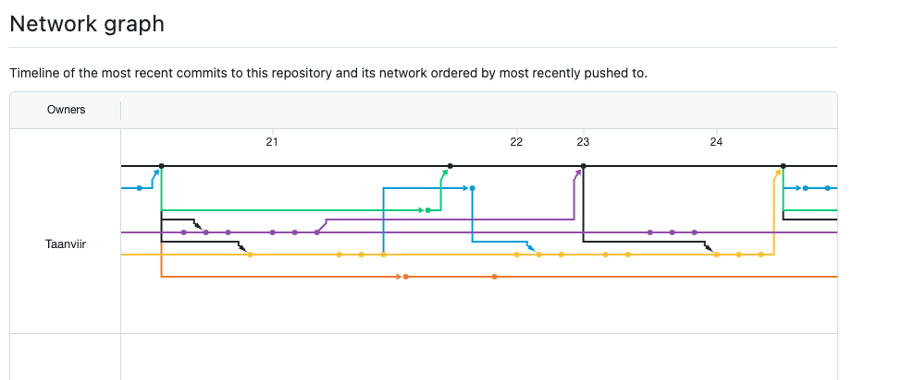
\includegraphics[width=1\linewidth]{./images/network-graph.png}
        \caption*{Network graph of GitHub, representing the main branch (black), fixes on the game (green), improvement of design of the pages (purple), and features of user management (yellow and blue).}
        \label{fig:network-grahp}
    \end{figure}
    \begin{figure}[H]
        % 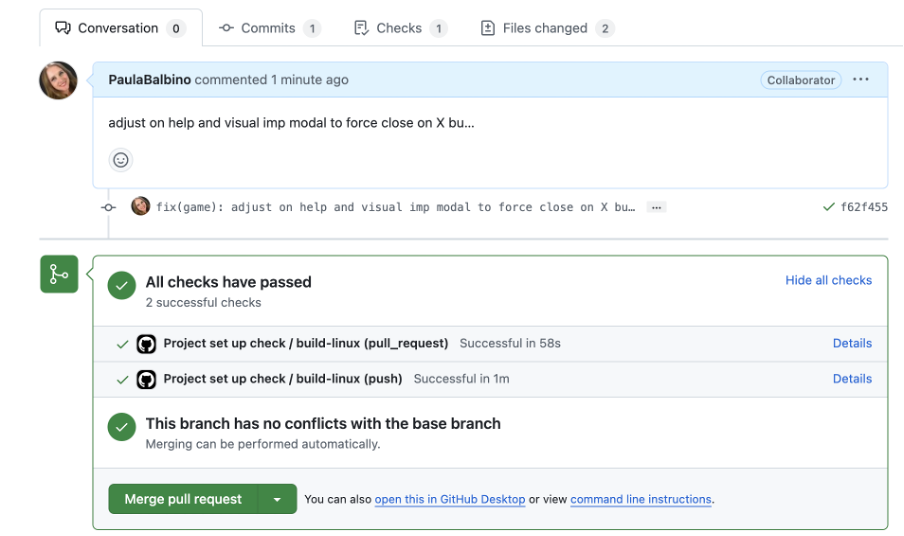
\includegraphics[width=1.0\linewidth]{images/ci-cd.png}
        \caption*{Continuous Integration and Continuous Deployment workflow used in the project. CI/CD integration on GitHub.}
        \label{fig:ci-cd}
    \end{figure}
    \begin{figure}[H]
        % 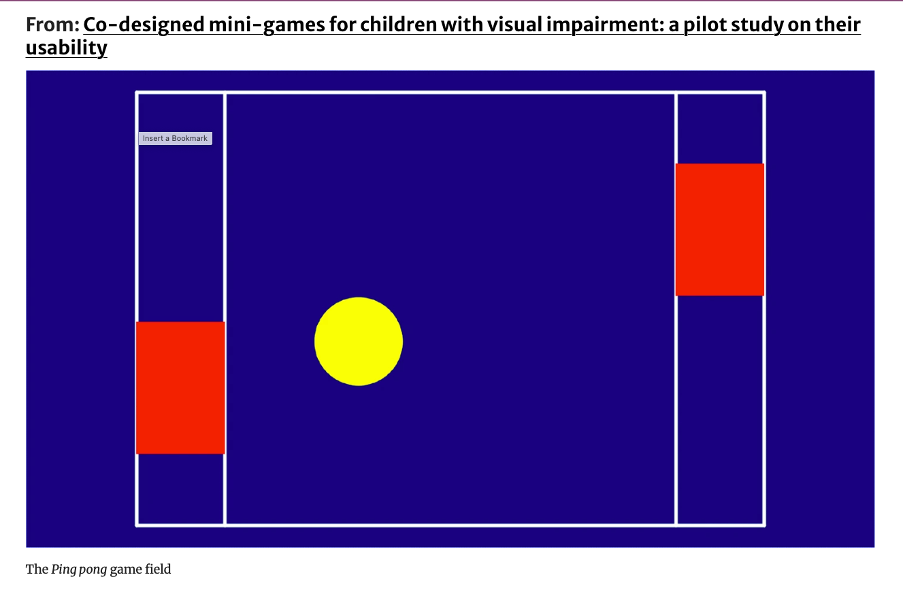
\includegraphics[width=1.0\linewidth]{images/vi-impairment.png}
        \caption*{The visual impairment mode of the project was inspired by the study Co-designed mini-games for children with visual impairment: A pilot study on their usability by Battistin et al. (2022), which explored accessible game design principles tailored for visually impaired children to enhance usability and engagement.}
        \label{fig:impairment}
    \end{figure}
\end{appendices}

\addcontentsline{toc}{section}{References}

\begin{thebibliography}{99}

\bibitem{intra-api}
42 (n.d.). Intra API documentation. Retrieved October 20, 2024, from \url{https://api.intra.42.fr/apidoc/guides/}

\bibitem{battistin2022}
Battistin, T., Dalla Pozza, N., Trentin, S., Volpin, G., Franceschini, A., \& Rodà, A. (2022). Co-designed mini-games for children with visual impairment: A pilot study on their usability. \textit{Multimedia Tools and Applications}. \url{https://doi.org/10.1007/s11042-022-13665-7}

\bibitem{bootstrap}
Bootstrap. (n.d.). Bootstrap documentation. Retrieved September 15, 2024, from \url{https://getbootstrap.com/docs}

\bibitem{django}
Django Software Foundation. (n.d.). Django documentation (version 5.0). Retrieved September 15, 2024, from \url{https://docs.djangoproject.com/en/5.0/}

\bibitem{django-otp}
Django OTP contributors. (n.d.). Django OTP documentation. Retrieved October 28, 2024, from \url{https://django-otp-official.readthedocs.io/en/latest/}

\bibitem{drf}
Encode OSS Ltd. (n.d.). Django REST framework documentation. Retrieved October 28, 2024, from \url{https://www.django-rest-framework.org/}

\bibitem{docker}
Docker Inc. (n.d.). Docker documentation. Retrieved October 28, 2024, from \url{https://docs.docker.com/}

\bibitem{ecma}
Ecma International. (n.d.). ECMAScript language specification. Retrieved September 25, 2024, from \url{https://www.ecma-international.org/publications-and-standards/}

\bibitem{elastic}
Elastic. (n.d.). Elastic Stack and Product Documentation. Retrieved October 28, 2024, from \url{https://www.elastic.co/guide/index.html}

\bibitem{geeksforgeeks}
GeeksforGeeks. (2024). What is single page application? Available at: \url{https://www.geeksforgeeks.org/what-is-single-page-application/}

\bibitem{guanabara_js}
Guanabara, G. (2019). Curso de JavaScript [Video]. YouTube. \url{https://www.youtube.com/watch?v=1-w1RfGIov4}

\bibitem{guanabara_html_css}
Guanabara, G. (2020). Curso de HTML e CSS [Video]. YouTube. \url{https://www.youtube.com/watch?v=1-w1RfGIov4}

\bibitem{mosh}
Programming with Mosh. (2021). Python Django tutorial for beginners [Video]. YouTube. \url{https://www.youtube.com/watch?v=rHux0gMZ3Eg}

\bibitem{nginx}
Nginx Inc. (n.d.). Nginx documentation. Retrieved October 28, 2024, from \url{https://nginx.org/en/docs/}

\bibitem{postgresql}
The PostgreSQL Global Development Group. (n.d.). PostgreSQL documentation. Retrieved October 26, 2024, from \url{https://www.postgresql.org/docs/current/}

\bibitem{simple_jwt}
Simple JWT. (n.d.). Simple JWT documentation. Retrieved October 18, 2024, from \url{https://django-rest-framework-simplejwt.readthedocs.io/en/latest/}

\bibitem{solidity}
Ethereum Foundation. (n.d.). Solidity documentation. Retrieved October 28, 2024, from \url{https://docs.soliditylang.org/}

\bibitem{stakeholdermap}
Stakeholdermap.com. (n.d.). Risk assessment matrix - Simple 3x3. Retrieved October 26, 2024, from \url{https://www.stakeholdermap.com/risk/risk-assessment-matrix-simple-3x3.html}

\bibitem{web3py}
Web3.py contributors. (n.d.). Web3.py documentation. Retrieved October 28, 2024, from \url{https://web3py.readthedocs.io/en/stable/}

\bibitem{wikipedia}
Wikipedia contributors. (n.d.). Single-page application. Wikipedia, The Free Encyclopedia. Retrieved September 8, 2024, from \url{https://en.wikipedia.org/wiki/Single-page_application}

\end{thebibliography}


% that's all folks :)

\end{document}  % The End
%% ----------------------------------------------------------------